\documentclass{book}
% Configuration
\usepackage[utf8]{inputenc}
%----------------
%   Imports
%----------------
\usepackage{xparse}
\usepackage{sectsty}
\usepackage[dvipsnames]{xcolor}
\usepackage{amsmath,amssymb,amsfonts,latexsym,cancel,amsthm,mathtools}


% \setlength{\parindent}{0cm}
% \setlength{\parskip}{5pt}

%-----------------
%   Colours
%-----------------
\definecolor{thmbg}{HTML}{F2F2F9}
\definecolor{lemmabg}{HTML}{FFFAF8}
\definecolor{lemmafr}{HTML}{983b0f}
\definecolor{propbg}{HTML}{f2fbfc}
\definecolor{propfr}{HTML}{191971}
\definecolor{myp}{RGB}{197, 92, 212}
\definecolor{primary}{HTML}{207ba5}    % Main colour
\definecolor{grey17}{RGB}{17, 17, 17}
\definecolor{greybg}{RGB}{249, 249, 249}
\definecolor{MyGrey}{HTML}{5B5B5B}

\definecolor{LightBlue}{rgb}{0.0, 0.64, 1.0}
\definecolor{LightRed}{rgb}{1.0, 0.50, 0.50}
\definecolor{DarkGreen}{rgb}{0.31, 0.54, 0.30}

%----------------
%	Text Styles
%----------------

\DeclareTextFontCommand{\term}{\color{orange}\itshape}
\DeclareTextFontCommand{\bred}{\color{red}\bfseries}
\DeclareTextFontCommand{\itblue}{\color{LightBlue}\itshape}

%----------------
%   URL Colour
%----------------
\usepackage[colorlinks=true]{hyperref}
\hypersetup{
    colorlinks=true,
    linkcolor=black,
    filecolor=magenta,
    urlcolor=blue,
}

%----------------
%   Boxes
%----------------

\usepackage[most]{tcolorbox}

\newcommand\fancybox[3]{%
    \tcbset{
        mybox/.style={
                enhanced,
                boxsep=0mm,
                opacityfill=0,
                overlay={
                        \coordinate (X) at ([xshift=-1mm, yshift=-1.5mm]frame.north west);
                        \node[align=right, text=#1, text width=2.5cm, anchor=north east] at (X) {\bf#2};
                        \draw[line width=0.5mm, color=#1] (frame.north west) -- (frame.south west);
                    }
            }
    }
    \begin{tcolorbox}[mybox]
        #3
    \end{tcolorbox}
}

\tcbuselibrary{theorems,skins,hooks}
\NewDocumentCommand\thmbox{m O{\Large #1} O{greybg} O{primary} O{number within=section}}
{
    \newtcbtheorem[#5]{#1}{\large #2}
    {%
        enhanced
        ,breakable
        ,colback = #3
        ,frame hidden
        ,boxrule = 0sp
        ,borderline west = {2pt}{0pt}{#4}
        ,sharp corners
        ,detach title
        ,before upper = \tcbtitle\par\smallskip
        ,coltitle = #4
        ,fonttitle = \bfseries
        % ,description font = \mdseries
        ,separator sign none
        ,segmentation style={solid, #4}
    }
    {th}
}

\thmbox{Corollary}[Corollary][myp!10][myp!85!black]
\thmbox{Lemma}[Lemma][lemmabg][lemmafr]
\thmbox{Propo}[Preposition][propbg][propfr]
\thmbox{defi}[Definition][primary!12][primary]
\thmbox{Notation}[Notation][white][grey17][no counter]
\thmbox{Theorem}[Theorem][primary!12][primary]

%---------------
%   Commands
%---------------
\newcommand{\theorem}[2]{\begin{Theorem}{#1}{}#2\end{Theorem}}
\newcommand{\corollary}[2]{\begin{Corollary}{#1}{}#2\end{Corollary}}
\newcommand{\lemma}[2]{\begin{Lemma}{#1}{}#2\end{Lemma}}
\newcommand{\proposition}[2]{\begin{Propo}{#1}{}#2\end{Propo}}
\newcommand{\notation}[2]{\begin{Notation}{#1}{}{\em\color{MyGrey}#2}\end{Notation}}
\newcommand{\definition}[2]{\begin{defi}{#1}{}#2\end{defi}}
\newcommand{\demonstration}[1]{\begin{proof}[\color{primary}\textbf{Demonstration.}] #1 \end{proof}}

\theoremstyle{definition}
\newtheorem*{exam}{\color{primary}Example}
\newcommand{\example}[1]{\begin{exam}#1\end{exam}}

\theoremstyle{definition}
\newtheorem*{solu}{\color{primary}Solution}
\newcommand{\solution}[1]{\begin{solu}#1\end{solu}}

\renewcommand{\qed}{\hfill$\blacksquare$}

%---------------
%   Lists
%---------------
\usepackage{tikz}

\usepackage{enumitem}

\newcommand{\cnumero}[2]{
    \tikz[baseline=(myanchor.base)]
    \node[minimum size=0.2cm,circle,
        inner sep=1pt,draw, #2,thick,fill=#2](myanchor)
    {\color{white}\bfseries\fontsize{8}{8}#1};}

\newcommand*{\itembolasazules}[1]{\protect\cnumero{#1}{primary}}

\newcommand{\listo}[1]{
    \begin{enumerate}[label=\itembolasazules{\arabic*}]
        #1
    \end{enumerate}
}

\newcommand{\listu}[1]{
    \begin{itemize}[label=$\color{primary} \bullet$]
        #1
    \end{itemize}
}

%-------------------------
% Table of Contents
%-------------------------

\usepackage{blindtext}
\usepackage{framed}
\usepackage{titletoc}
\usepackage{etoolbox}

\patchcmd{\tableofcontents}{\contentsname}{\contentsname}{}{}

\renewenvironment{leftbar}
{\def\FrameCommand{\hspace{6em}%
        {\color{primary}\vrule width 2pt depth 6pt}\hspace{1em}}%
    \MakeFramed{\parshape 1 0cm \dimexpr\textwidth-6em\relax\FrameRestore}\vskip2pt%
}
{\endMakeFramed}

\titlecontents{chapter}[0em]
{\vspace*{2\baselineskip}}
{\parbox{4.5em}{%
        \hfill\Huge\bfseries\color{primary}\thecontentslabel}%
    \vspace*{-2.3\baselineskip}\leftbar\textbf{\color{primary}\small\chaptername~\thecontentslabel}\\
}{}{\endleftbar}

\titlecontents{section}[8.4em]
{\contentslabel{3em}}{}{}
{\hspace{0.5em}\nobreak\itshape\color{primary}\contentspage}

\titlecontents{subsection}[8.4em]
{\contentslabel{3em}}{}{}
{\hspace{0.5em}\nobreak\itshape\color{primary}\contentspage}

%-----------------------------
%   Chapter formats
%-----------------------------

%==================
% Chapters
%==================
\newtcolorbox{titlecolorbox}[1]{ %the box around chapter
    coltext=white,
    colframe=primary,
    colback=primary,
    boxrule=0pt,
    arc=0pt,
    notitle,
    width=4.8em,
    height=2.4ex,
    before=\hfill
}

\usepackage[explicit]{titlesec}

\makeatletter
\let\old@rule\@rule
\def\@rule[#1]#2#3{\textcolor{primary}{\old@rule[#1]{#2}{#3}}}
\makeatother

\titleformat{\chapter}[display]
{\Huge}
{}
{0pt}
{\begin{titlecolorbox}{}
        {\large\MakeUppercase{\bf\chaptername}}
    \end{titlecolorbox}
    \vspace*{-3.19ex}\noindent\rule{\textwidth}{0.4pt}
    \parbox[b]{\dimexpr\textwidth-4.8em\relax}{\raggedright\MakeUppercase{#1}}{\hfill\fontsize{70}{60}\selectfont{\color{primary}\thechapter}}
}
[]

\titleformat{name=\chapter,numberless}[display]
{\Huge}
{}
{0pt}
{
    \vspace*{-3.19ex}\noindent\rule{\textwidth}{0.4pt}
    \parbox[b]{\dimexpr\textwidth-4.8em\relax}{\raggedright\MakeUppercase{#1}}
}
[]

%==============
% Sections
%==============

\titleformat{\section}[hang]{\Large\bfseries}%
{\rlap{\color{primary}\rule[-6pt]{\textwidth}{0.4pt}}\colorbox{primary}{%
        \raisebox{0pt}[13pt][3pt]{ \makebox[60pt]{% height, width
                \selectfont\color{white}{\thesection}}
        }}}%
{15pt}%
{ \color{primary}#1
    %
}
\titlespacing*{\section}{0pt}{3mm}{5mm}

%================
% Sub sections
%================
\subsectionfont{\Large\color{primary}}


%-----------------
%	BIBLIOGRAPHY AND INDEX
%-----------------

\usepackage{csquotes}
\usepackage[style=alphabetic,citestyle=numeric,sorting=nyt,sortcites=true,autopunct=true,autolang=hyphen,hyperref=true,abbreviate=false,backref=true,backend=biber,defernumbers=true]{biblatex}
\addbibresource{./bibliography.bib} % BibTeX bibliography file
\defbibheading{bibempty}{}

\usepackage{calc} % For simpler calculation - used for spacing the index letter headings correctly
\usepackage{makeidx} % Required to make an index
\makeindex % Tells LaTeX to create the files required for indexing

%---------------------
% Front page
%---------------------
\usetikzlibrary{ shapes.geometric }
\usetikzlibrary{calc}
\usepackage{anyfontsize}
\newcommand{\portada}[3]{
    \begin{tikzpicture}[remember picture,overlay]
        %%%%%%%%%%%%%%%%%%%% Background %%%%%%%%%%%%%%%%%%%%%%%%
        \fill[primary] (current page.south west) rectangle (current page.north east);


        \foreach \i in {2.5,...,22}
            {
                \node[rounded corners,primary!60,draw,regular polygon,regular polygon sides=6, minimum size=\i cm,ultra thick] at ($(current page.west)+(2.5,-5)$) {} ;
            }

        %%%%%%%%%%%%%%%%%%%% Background Polygon %%%%%%%%%%%%%%%%%%%% 
        \foreach \i in {0.5,...,22}
            {
                \node[rounded corners,primary!60,draw,regular polygon,regular polygon sides=6, minimum size=\i cm,ultra thick] at ($(current page.north west)+(2.5,0)$) {} ;
            }

        \foreach \i in {0.5,...,22}
            {
                \node[rounded corners,primary!90,draw,regular polygon,regular polygon sides=6, minimum size=\i cm,ultra thick] at ($(current page.north east)+(0,-9.5)$) {} ;
            }


        \foreach \i in {21,...,6}
            {
                \node[primary!85,rounded corners,draw,regular polygon,regular polygon sides=6, minimum size=\i cm,ultra thick] at ($(current page.south east)+(-0.2,-0.45)$) {} ;
            }


        %%%%%%%%%%%%%%%%%%%% Title %%%%%%%%%%%%%%%%%%%% 
        \node[left,primary!5,minimum width=0.625*\paperwidth,minimum height=3cm, rounded corners] at ($(current page.north east)+(0,-9.5)$)
        {
            {\fontsize{25}{30} \selectfont \bfseries #1}
        };

        %%%%%%%%%%%%%%%%%%%% Subtitle %%%%%%%%%%%%%%%%%%%% 
        \node[left,primary!10,minimum width=0.625*\paperwidth,minimum height=2cm, rounded corners] at ($(current page.north east)+(0,-11)$)
        {
            {\huge \textit{#2}}
        };

        %%%%%%%%%%%%%%%%%%%% Author Name %%%%%%%%%%%%%%%%%%%% 
        \node[left,primary!5,minimum width=0.625*\paperwidth,minimum height=2cm, rounded corners] at ($(current page.north east)+(0,-13)$)
        {
            {\Large \textsc{#3}}
        };

        %%%%%%%%%%%%%%%%%%%% Year %%%%%%%%%%%%%%%%%%%% 
        \node[rounded corners,fill=primary!70,text =primary!5,regular polygon,regular polygon sides=6, minimum size=2.5 cm,inner sep=0,ultra thick] at ($(current page.west)+(2.5,-5)$) {\LARGE \bfseries \the\year{}};

    \end{tikzpicture}
}
\usepackage[letterpaper]{geometry}
\usepackage{graphicx, wrapfig, subcaption, setspace, booktabs}
\usepackage[T1]{fontenc}
\usepackage{babel}
\usepackage[scaled]{helvet}     % Document source
%\renewcommand{\familydefault}{\sfdefault}
\usepackage{url, lipsum}
\usepackage{tabularx}

% You can change the main color
% \definecolor{primary}{HTML}{}

\begin{document}

\pagestyle{empty}
\portada{CSC263}{Data Structures and Analysis}{Sinan Li}
\newpage

\tableofcontents

\newpage

\part{Data Structure}

\chapter{Priority Queues and Heaps}

\begin{minipage}[t]{0.45\linewidth}
    \textbf{Data}
    
    \listu{
        \item Collection of elements
    
        \item Each element $x$ has a priority 
        
        $x$.\textit{priority}
    }
\end{minipage}
\begin{minipage}[t]{0.45\linewidth}
    \textbf{Operations}
    
    \listu{
        \item \textsc{Insert}$(Q, x)$
        
        Add $x$ to $Q$ 
        
        Note: $x$.\textit{priority} can be non-unique

        \item \textsc{Max}$(Q)$
        
        Return the element with max priority

        Note: $Q$ is unchanged

        \item \textsc{Extract-Max}$(Q)$
        
        Remove and return the element with the max priority
    }
\end{minipage}

\section{Implementation}

\subsection{Attempts}

\subsubsection{Implementation 1: Unsorted Array / Linked List}

\begin{itemize}
    \item \textsc{Insert} takes $\Theta(1)$ time in the worst case 
    \item \textsc{Max} takes $\Theta(n)$ time in the worst case 
    \item \textsc{ExtractMax} takes $\Theta(n)$ time in the worst case
\end{itemize}

\subsubsection{Implementation 2: Sorted Array / Linked List}

\begin{itemize}
    \item \textsc{Insert} takes $\Theta(n)$ time in the worst case 
    \item \textsc{Max} takes $\Theta(1)$ time in the worst case 
    \item \textsc{ExtractMax} takes $\Theta(1)$ time in the worst case
\end{itemize}

\subsection{Implementation}

We want to combine the advantages of both data structures by having a ``partially sorted'' ADT -- a (binary) \term{heap}\index{Heap}. 

There are two kinds of binary heaps: max-heaps and min-heaps. In both kinds, the values in the nodes satisfy a \bred{heap property}, the specifics of which depend on the kind of heap. 

\begin{itemize}
    \item Max heap property: the key of every node $x$ is \itblue{larger} than or equal to the keys of its children. 
    
    The largest element in a max-heap is stored at the root.
    
    \item Min heap property: the key of every node $x$ is \itblue{smaller} than or equal to the keys of its children
    
    The smallest element in a min-heap is stored at the root,
\end{itemize}

These are called \term{heap orders}. There is no ordering between the siblings. A max/min heap is valid if it is a nearly complete binary tree and it satisfies the max/min heap property.

\begin{figure}[ht!]
    \tikzset{
        every node/.style = {draw, circle, minimum size=2em}, 
        level 1/.style={sibling distance=6em}, 
        level 2/.style={sibling distance=3em}, 
        level 3/.style={sibling distance=1.5em}
    }
    \centering
    \begin{tikzpicture}
        \node {$17$}
        child {
            node {$12$}
            child { node {$5$} }
            child { node {$8$} }
        }
        child {node {$2$} };
    \end{tikzpicture}
    \hfill
    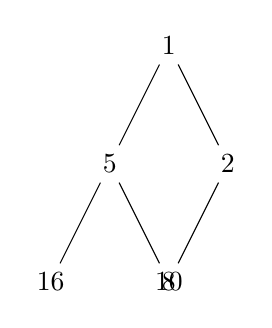
\begin{tikzpicture}
        \node {$1$}
        child {
            node {$5$}
            child { node {$16$} }
            child { node {$8$} }
        }
        child {node {$2$} 
            child { node {$10$} }
            child[missing]
        };
    \end{tikzpicture}
    \hfill
    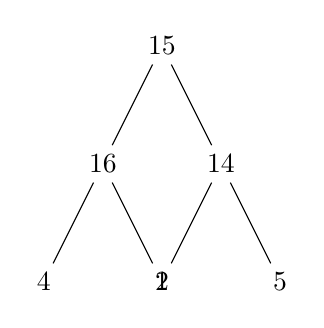
\begin{tikzpicture}
        \node {$15$}
        child {
            node {$16$}
            child { node {$4$} }
            child { node {$2$} }
        }
        child {node {$14$} 
            child { node {$1$} }
            child { node {$5$} }
        };
    \end{tikzpicture}
    \caption{A valid max-heap (left), a valid min-heap (middle), and an invalid heap (right)}
\end{figure}

Although a heap is an \bred{almost complete binary tree} \footnote{That is, the tree is completely filled on all levels except possibly the lowest, which is filled from the left up to a point. }, in practice, we usually use an array to store the data in memory. An array $H$ that represents a heap is an object with two attributes: $H$.\textit{length}, which (as usual) gives the number of elements in the array, and $H$.\textit{heap-size}, which represents how many elements in the heap are stored within array $H$. The root of the tree is $H[1]$, and given the index $i$ of a node, we can compute the indices of its parent, left child, and right child:

\begin{minipage}[t]{0.3\linewidth} \begin{itemize}
    \item \textsc{Parent}
    
    \textbf{return} $\lfloor i / 2 \rfloor$
\end{itemize} \end{minipage}
\begin{minipage}[t]{0.3\linewidth} \begin{itemize}
    \item \textsc{Left}
    
    \textbf{return} $2i$
\end{itemize} \end{minipage}
\begin{minipage}[t]{0.3\linewidth} \begin{itemize}
    \item \textsc{Right}

    \textbf{return} $2i + 1$
\end{itemize} \end{minipage}

\section{Operations}
\subsection{\textsc{Insert}}

To insert element with key $p$ into the heap $H$, 

\listu{
    \item Increment $H$.\textit{heap-size} and add a new node with key $p$ to the next available position

    \item Repeatedly swap the new item with its parent until the heap property is satisfied

    This swapping process is called \bred{bubbling up}

    \item Worst-case runtime: $\Theta(\lg n)$
}

{~~~}

For example, consider \textsc{Insert}$(H, 17)$ where $H = [16, 8, 10, 1, 5, 3]$

\begin{minipage}[t]{0.3\linewidth} \begin{center} \begin{tikzpicture} [
    every node/.style = {circle, fill=Violet, minimum size=2em}, 
    level 1/.style={sibling distance=6em}, 
    level 2/.style={sibling distance=3em}, 
    level 3/.style={sibling distance=1.5em},
    baseline=(current bounding box.north)
]
    \node {$16$} 
    child {
        node {$8$} 
        child { node {$1$} }
        child { node {$5$} }
    }
    child {
        node {$10$}
        child { node {$3$} }
        child { node [fill=MyRed] {$17$} }
    };
\end{tikzpicture} \end{center} \end{minipage}
\begin{minipage}[t]{0.3\linewidth} \begin{center} \begin{tikzpicture} [
    every node/.style = {circle, fill=Violet, minimum size=2em}, 
    level 1/.style={sibling distance=6em}, 
    level 2/.style={sibling distance=3em}, 
    level 3/.style={sibling distance=1.5em},
    baseline=(current bounding box.north)
]
    \node {$16$} 
    child {
        node {$8$} 
        child { node {$1$} }
        child { node {$5$} }
    }
    child { 
        node [fill=MyRed] (17) {$17$}
        child { node {$3$} }
        child { node (10) {$10$} }
    };

    \draw[bend left=60, dashed,latex-latex,color=MyRed]  (17) to (10);
\end{tikzpicture} \end{center} \end{minipage}
\begin{minipage}[t]{0.3\linewidth} \begin{center} \begin{tikzpicture} [
    every node/.style = {circle, fill=Violet, minimum size=2em}, 
    level 1/.style={sibling distance=6em}, 
    level 2/.style={sibling distance=3em}, 
    level 3/.style={sibling distance=1.5em},
    baseline=(current bounding box.north)
]
    \node [fill=MyRed] (17) {$17$}
    child {
        node {$8$} 
        child { node {$1$} }
        child { node {$5$} }
    }
    child { 
        node (16) {$16$}     
        child { node {$3$} }
        child { node {$10$} }
    };

    \draw[bend left=60, dashed,latex-latex,color=MyRed]  (17) to (16);
\end{tikzpicture} \end{center} \end{minipage}

\begin{algorithm}[H] \begin{algorithmic}
    \Procedure{Max-Heap-Insert}{$H$, $p$}
        \State $i \gets H.\textit{heap-size} \gets H.\textit{heap-size} + 1$
        \State $H[i] = p$
        \While{$\textsc{Parent}(i) > 0$ \textbf{and} $H[i] > H[\textsc{Parent}(i)]$}
            \State swap $H[i]$ with $H[\textsc{Parent}[i]]$
            \State $i \gets \textsc{Parent}(i)$
        \EndWhile
    \EndProcedure
\end{algorithmic} \end{algorithm}

\subsection{\textsc{Find-Max}}

To find the maximum key in the heap $H$, 

\listu{
    \item Simply return the item in the root

    \item Worst-case runtime: $\Theta(1)$
}

\begin{center} \begin{tikzpicture} [
    every node/.style = {circle, fill=Violet, minimum size=2em}, 
    level 1/.style={sibling distance=6em}, 
    level 2/.style={sibling distance=3em}, 
    level 3/.style={sibling distance=1.5em},
    baseline=(current bounding box.north)
]
    \node (root) {$17$}
    child {
        node {$8$} 
        child { node {$1$} }
        child { node {$5$} }
    }
    child { 
        node (16) {$16$}     
        child { node {$3$} }
        child { node {$10$} }
    };
    
    \draw[bend left=30, dashed, -latex, color=MyRed] (-1.25,0.5) to (-0.25,0.5);
\end{tikzpicture} \end{center}

\begin{algorithm}[H] \begin{algorithmic}[1]
    \Procedure{Find-Max}{$H$}
        \State \Return $H[1]$
    \EndProcedure
\end{algorithmic} \end{algorithm}

\subsection{\textsc{Extract-Max}}

\listu {
    \item Save the item from the root in a temporary variable
    \item Replace the root with the rightmost item in the lowest level of the tree and decrement $H$.\textit{heap-size}
    \item Repeatedly swap the item we moved with its largest child until the heap property is restored. This swapping process is called \bred{bubble down}.
    \item Worst-case runtime: $\Theta(\lg n)$
}

\begin{minipage}[t]{0.32\linewidth} \begin{center} \begin{tikzpicture} [
    every node/.style = {circle, fill=Violet, minimum size=2em}, 
    level 1/.style={sibling distance=6em}, 
    level 2/.style={sibling distance=3em}, 
    level 3/.style={sibling distance=1.5em},
    baseline=(current bounding box.north)
]
    \node[fill=MyRed] (root) {$17$}
    child {
        node {$8$} 
        child { node {$1$} }
        child { node {$5$} }
    }
    child { 
        node (16) {$16$}     
        child { node {$3$} }
        child { node {$10$} }
    };

    \node[left of=root, node distance=2cm] (17) {$17$};
    
    \draw[dashed, -latex, color=MyRed] (root) to (17);
    \draw[bend right=60, dashed, -latex, color=MyRed] (10) to (root);
\end{tikzpicture} \end{center} \end{minipage}
\begin{minipage}[t]{0.32\linewidth} \begin{center} \begin{tikzpicture} [
    every node/.style = {circle, fill=Violet, minimum size=2em}, 
    level 1/.style={sibling distance=6em}, 
    level 2/.style={sibling distance=3em}, 
    level 3/.style={sibling distance=1.5em},
    baseline=(current bounding box.north)
]
    \node[fill=MyRed] (root) {$10$}
    child {
        node {$8$} 
        child { node {$1$} }
        child { node {$5$} }
    }
    child { 
        node (16) {$16$}     
        child { node {$3$} }
        child[missing]
    };
    
    \draw[bend left=60, dashed, latex-latex, color=MyRed] (root) to (16);
\end{tikzpicture} \end{center} \end{minipage}
\begin{minipage}[t]{0.32\linewidth} \begin{center} \begin{tikzpicture} [
    every node/.style = {circle, fill=Violet, minimum size=2em}, 
    level 1/.style={sibling distance=6em}, 
    level 2/.style={sibling distance=3em}, 
    level 3/.style={sibling distance=1.5em},
    baseline=(current bounding box.north)
]
    \node (root) {$16$}
    child {
        node {$8$} 
        child { node {$1$} }
        child { node {$5$} }
    }
    child { 
        node[fill=MyRed] (10) {$10$}     
        child { node {$3$} }
        child[missing]
    };
    
    \draw[bend left=60, dashed, latex-latex, color=MyRed] (root) to (16);
\end{tikzpicture} \end{center} \end{minipage}

\begin{algorithm}[H] \begin{algorithmic}[1]
    \Procedure{Extract-Max}{$H$}
        \State $\textit{max} \gets H[1]$

        \State $H[1] \gets H[H.\textit{heap-size}]$

        \State $H.\textit{heap-size} \gets H.\textit{heap-size} - 1$

        \State \textsc{Max-Heapify}$(H, 1)$

        \State \textbf{return} \textit{max}
    \EndProcedure
\end{algorithmic} \end{algorithm}

\begin{algorithm}[H] \begin{algorithmic}[1]
    \Procedure{Max-Heapify}{$H$, $i$}
        \State $l \gets \textsc{Left}(i)$
        \State $r \gets \textsc{Right}(i)$

        \If {$l \leq H.\textit{heap-size}$ \textbf{and} $H[l] > H[i]$}
            \State $\textit{largest} \gets l$
        \Else
            \State $\textit{largest} \gets i$
        \EndIf

        \If {$r \leq H.\textit{heap-size}$ \textbf{and} $H[r] > H[\textit{largest}]$}
            \State $\textit{largest} \gets r$
        \EndIf

        \If {$\textit{largest} \neq i$}
            \State swap $H[i]$ with $H[\textit{largest}]$
            \State \textsc{Max-Heapify}$(H, \textit{largest})$
        \EndIf
    \EndProcedure
\end{algorithmic} \end{algorithm}

\subsection{\textsc{Build-Max-Heap}}

\listu {
    \item Takes an array $A$ of length $n$ and builds a max-heap $H$ from it.
    \item Worst-case runtime: $\Theta(n)$
}

\begin{algorithm}[H] \begin{algorithmic}[1]
    \Procedure{Build-Max-Heap}{$A$}
        \State $H.\textit{heap-size} \gets A.\textit{length}$
        \For {$i = \lfloor \frac{A.\textit{length}}{2} \rfloor$ \textbf{downto} $1$}
            \State \textsc{Max-Heapify}$(H, i)$
        \EndFor
    \EndProcedure
\end{algorithmic} \end{algorithm}
\chapter{Dictionary}

\begin{minipage}[t]{0.45\linewidth}
    \textbf{Data}

    \listu {
        \item A set $S$
        \item Each element $x$ has a \bred{unique} key $x$.\textit{key}
    }
\end{minipage}
\begin{minipage}[t]{0.45\linewidth}
    \textbf{Operations}

    \listu { 
        \item \textsc{Search}$(S, k)$
        
        Return $x$ in $S$ with $x.\textit{key} = k$ (or NIL).

        \item \textsc{Insert}$(S, x)$
        
        Add $x$ to $S$ -- if $S$ contains $y$ with $y.\textit{key} = x.\textit{key}$, then \itblue{replace} $y$ with $x$.

        \item \textsc{Delete}$(S, x)$ \footnote{If we are given the key $k$ instead of the element $x$, we could do \textsc{Delete}$(S, \textsc{Search}$(S, k)$)$}
        
        Remove element $x$ from $S$.
    }
\end{minipage}

\begin{table}[H]
    \centering
    \begin{tabular}{r | c c c}                                                                   \hline
                               & \textsc{Search}   & \textsc{Insert}   & $\textsc{Delete}^\#$ \\ \hline
        unsorted array         & $n$               & $n$               & $1$                  \\
        sorted$^*$ array       & $\lg n$           & $n$               & $n$                  \\
        unsorted linked list   & $n$               & $n$               & $1$                  \\
        sorted$^*$ linked list & $n$               & $n$               & $1$                  \\ \hline
        direct access table    & $1$               & $1$               & $1$                  \\
        hash table             & $n$               & $n$               & $n$                  \\ \hline
        binary search tree     & height of the BST & height of the BST & height of the BST    \\
        balanced search tree   & $\lg n$           & $\lg n$           & $\lg n$              \\ \hline
    \end{tabular}
\end{table}


$^*$: these require the keys to be ordered

$^\#$: here we are only doing deletion (without having to search for $x$)

\section{Binary Search Tree}\index{Binary Search Tree}

A binary search tree is a binary tree with the \term{binary-search-tree property}\index{Binary Search Tree!Binary-Search-Tree Property}:

\textit{Let $x$ be a node in a binary search tree. If $y$ is a node in the left subtree of $x$, then $y.\textit{key} \leq x.\textit{key}$. If $y$ is a node in the right subtree of $x$, then $y.\textit{key} \geq x.\textit{key}$.}

\begin{figure}[H]
    \tikzset{
        every node/.style = {draw, circle, minimum size=2em}, 
        level 1/.style={sibling distance=6em}, 
        level 2/.style={sibling distance=3em}, 
        level 3/.style={sibling distance=1.5em}
    }
    \centering
    \begin{tikzpicture}
        \node {$17$}
        child {
            node {$8$}
            child { node {$5$} }
            child { node {$12$} }
        }
        child {node {$21$} 
            child[missing]
            child { node {$23$} }
        };
    \end{tikzpicture}
    \hfill
    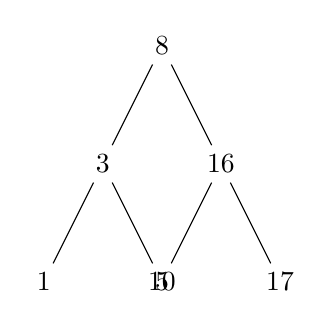
\begin{tikzpicture}
        \node {$8$}
        child {
            node {$3$}
            child { node {$1$} }
            child { node {$5$} }
        }
        child {node {$16$} 
            child { node {$10$} }
            child { node {$17$} }
        };
    \end{tikzpicture}
    \hfill
    \begin{tikzpicture}
        \node {$15$}
        child {
            node {$6$}
            child { node {$3$} }
            child { 
                node {$7$} 
                child[missing]
                child { node {$13$} }
            }
        }
        child {node {$18$} 
            child[missing]
            child { node {$20$} }
        };
    \end{tikzpicture}
    \caption{Examples of binary search trees}
\end{figure}

\begin{minipage}[t]{0.32\linewidth}
    \begin{verbatim}
class Item:
    key: Any
    value: Any
    \end{verbatim}
\end{minipage}
\begin{minipage}[t]{0.32\linewidth}
    \begin{verbatim}
class BST_Node:
    item: Item 
    left: BST_Node
    right: BST_Node
    \end{verbatim}
\end{minipage}
\begin{minipage}[t]{0.32\linewidth}
    \begin{verbatim}
class Dictionary:
    root: BST_Node
    \end{verbatim}
\end{minipage}

\subsection{\textsc{Insert}}

\begin{minipage}[t]{0.425\linewidth} \begin{algorithm}[H] \begin{algorithmic}[1]
    \Procedure{Insert}{$S$, $x$}
        \State $S.\textit{root} \gets \textsc{BST-Insert}(S.\textit{root}, x)$
    \EndProcedure
\end{algorithmic} \end{algorithm} \end{minipage}
\hfill
\begin{minipage}[t]{0.525\linewidth} \begin{algorithm}[H] \begin{algorithmic}[1]
    \Procedure{BST-Insert}{\textit{root}, $x$}
        \State \cmt{Insert $x$ into stubree at root; return new root}
        \If {$\textit{root} = \text{NIL}$}
            \State $\textit{root} \gets \textsc{BST\_Node}(x)$ \cmt{Add $x$}
        \ElsIf {$x.\textit{key} < \textit{root.item.key}$}
            \State $\textit{root.left} \gets \textsc{BST-Insert}(\textit{root.left}, x)$
        \ElsIf {$x.\textit{key} > \textit{root.item.key}$}
            \State $\textit{root.right} \gets \textsc{BST-Insert}(\textit{root.right}, x)$
        \Else {~} \cmt{$x.\textit{key} = \textit{root.item.key}$}
            \State $\textit{root.item} \gets x$ \cmt{replace with $x$}
        \EndIf
        \State \Return $\textit{root}$
    \EndProcedure
\end{algorithmic} \end{algorithm} \end{minipage}

\subsection{\textsc{Search}}

\begin{minipage}[t]{0.425\linewidth} \begin{algorithm}[H] \begin{algorithmic}[1]
    \Procedure{Search}{$S$, $k$}
        \State $\textit{node} \gets \textsc{BST-Search}(S.\textit{root}, k)$
        \If {$\textit{node} = \text{NIL}$}
            \State \Return $\text{NIL}$
        \EndIf
        \State \Return $\textit{node.item}$
    \EndProcedure
\end{algorithmic} \end{algorithm} \end{minipage}
\hfill
\begin{minipage}[t]{0.525\linewidth} \begin{algorithm}[H] \begin{algorithmic}[1]
    \Procedure{BST-Search}{\textit{root}, $k$}
        \State \cmt{Return node under root with key $k$ (or NIL)}
        \If {$\textit{root} = \text{NIL}$}
            \State pass \cmt{$k$ not in tree}
        \ElsIf {$k < \textit{root.item.key}$}
            \State $\textit{root} \gets \textsc{BST-Search}(\textit{root.left}, k)$
        \ElsIf {$k > \textit{root.item.key}$}
            \State $\textit{root} \gets \textsc{BST-Search}(\textit{root.right}, k)$
        \Else {~} \cmt{$k = \textit{root.item.key}$}
            \State pass
        \EndIf
        \State \Return $\textit{root}$
    \EndProcedure
\end{algorithmic} \end{algorithm} \end{minipage}

\subsection{\textsc{Delete}}

\begin{algorithm}[H] \begin{algorithmic}[1]
    \Procedure{Delete}{$S$, $k$}
        \State $S.\textit{root} \gets \textsc{BST-Delete}(S.\textit{root}, k)$
    \EndProcedure
\end{algorithmic} \end{algorithm}

\begin{algorithm}[H] \begin{algorithmic}[1]
    \Procedure{BST-Delete}{\textit{root}, $x$}
        \State \cmt{Delete $x$ from stubree at root; return new root}
        \If {$\textit{root} = \text{NIL}$}
            pass \cmt{$x$ not in tree}
        \ElsIf {$x < \textit{root.item.key}$}
            \State $\textit{root.left} \gets \textsc{BST-Delete}(\textit{root.left}, x)$
        \ElsIf {$x > \textit{root.item.key}$}
            \State $\textit{root.right} \gets \textsc{BST-Delete}(\textit{root.right}, x)$
        \Else {~} \cmt{$x.\textit{key} = \textit{root.item.key}$}
            \If {$\textit{root.left} = \text{NIL}$}
                \State $\textit{root} \gets \textit{root.right}$ \cmt{could be NIL}
            \ElsIf {$\textit{root.right} = \text{NIL}$}
                \State $\textit{root} \gets \textit{root.left}$
            \Else {~} \cmt{Replace \textit{root.item} with its successor}
                \State $\textit{root.item}, \textit{root.right} \gets \textsc{BST-Del-Min}(\textit{root.right})$
            \EndIf
        \EndIf
        \State \Return $\textit{root}$
    \EndProcedure
\end{algorithmic} \end{algorithm}

\begin{algorithm}[H] \begin{algorithmic}[1]
    \Procedure{BST-Del-Min}{\textit{root}}
        \State \cmt{Remove element with smallest key under root; return item and root of resulting subtree}
        \Require $\textit{root} \neq \text{NIL}$

        \If {$\textit{root.left} = \text{NIL}$}
            \State \Return $\textit{root.item}, \textit{root.right}$
        \Else 
            \State $\textit{item}, \textit{root.left} \gets \textsc{BST-Del-Min}(\textit{root.left})$
            \State \Return $\textit{item}, \textit{root}$
        \EndIf
    \EndProcedure
\end{algorithmic} \end{algorithm}

\section{Balanced Search tree}

Despite the simplicity of the BST, it is not a very efficient data structure. The worst-case running time of the BST operations is proportional to the height of the tree, which is $\Theta(n)$, where $n$ is the number of elements in the tree. The shape of a BST is determined by the order in which keys are inserted. If the keys are inserted in sorted order, the BST degenerates into a linked list. 

We can improve the performance of the BST by making it more balanced. A \term{balanced BST}\index{Balanced Binary Search Tree} (also known as an \term{AVL tree}\index{AVL Tree} -- Adelson-Velsky, Landis Tree) is one in which the heights of the two subtrees of any node differ by at most one. The height of a balanced BST is $\Theta(\log n)$, where $n$ is the number of elements in the tree.

\begin{figure}[H]
    \centering
    \begin{tikzpicture}[level 1/.style={sibling distance=16em}, 
        level 2/.style={sibling distance=8em}, 
        level 3/.style={sibling distance=4em}
    ]
        \node[draw, circle] {$21$} 
        child{ node[draw, circle]{$2$} 
            child {node[draw, circle] {$1$} 
                child{ node[draw, color=red, isosceles triangle, rotate=90, minimum size=1em] {} edge from parent[red,dashed] }
                child{ node[draw, color=red, isosceles triangle, rotate=90, minimum size=1em] {} edge from parent[red,dashed] }
            }
            child {node[draw, circle] {$13$} 
                child { node[draw, circle] {$5$} 
                    child{ node[draw, color=red, isosceles triangle, rotate=90, minimum size=1em] {} edge from parent[red,dashed] }
                    child{ node[draw, color=red, isosceles triangle, rotate=90, minimum size=1em] {} edge from parent[red,dashed] }
                }
                child { node[draw, color=red, isosceles triangle, rotate=90, minimum size=1em] {} edge from parent[red,dashed] }
            }
        }
        child { node[draw, circle] {$55$ }
            child { node[draw, circle] {$34$} 
                child{ node[draw, color=red, color=red, isosceles triangle, rotate=90, minimum size=1em] {} edge from parent[red,dashed] }
                child{ node[draw, color=red, color=red, isosceles triangle, rotate=90, minimum size=1em] {} edge from parent[red,dashed] }
            }
            child{ node[draw, color=red, isosceles triangle, rotate=90, minimum size=1em] {} edge from parent[red,dashed] }
        };
    \end{tikzpicture}
    \caption{AVL balanced binary search tree}
\end{figure}

To implement an AVL tree, we need a mechanism to detect imbalance in the tree, and a way to restore balance. We will use the following definition of \term{balance factor}\index{Balance Factor} of a node $x$ in a BST:

\definition{Balance Factor\index{AVL Tree!Balance Factor}} {
    An AVL balanced node $x$ has a balance factor of $-1$, $0$, or $1$. If the height of its left subtree is $h_L$, and the height of its right subtree is $h_R$, then $x$ has a balance factor of $h_L - h_R$.

    \listu {
        \item If $h_R - h_L = 0$, then $x$ is balanced.
        \item If $h_R - h_L = 1$, then $x$ is right-heavy.
        \item If $h_R - h_L = -1$, then $x$ is left-heavy.
    }
}

\begin{figure}[H]
    \tikzset{
        every node/.style={circle, minimum size=2em, fill=Violet},
        level 1/.style={sibling distance=10em},
        level 2/.style={sibling distance=5em},
        level 3/.style={sibling distance=2.5em}
    }
    \begin{tikzpicture}
        \node {}
        child {
            node {}
            child { node {} }
            child { 
                node {} 
                child[missing]
                child { node {} }
            }
        }
        child {
            node {}
            child { node {} }
            child { node {} }
        };
    \end{tikzpicture}
    \hfill
    \begin{tikzpicture}
        \node{} 
        child {
            node[fill=red!50] {}
            child { 
                node {} 
                child { node {} }
                child[missing]
            }
            child[missing]
        }
        child {
            node {}
            child { 
                node {} 
                child[missing]
                child { node {} }
            }
            child { node {} }
        }
        ;
    \end{tikzpicture}
    \caption{AVL balanced tree (left) and unbalanced tree (right)}
\end{figure}

\subsubsection{Rotations}

To restore balance, we need to perform a \term{rotation}\index{AVL Tree!Rotation} on the tree. There are four types of rotations, depending on the balance factor of the node and its children. The following figure shows the four types of rotations.

\begin{minipage}[t]{0.45\linewidth} \begin{figure}[H]
    \tikzset{
        baseline = (current bounding box.center),
        every node/.style={circle, minimum size=2em, fill=Violet},
        level distance=4em
    }
    \centering
    \begin{tikzpicture}
        \node {$x$}
        child { node {$y$}
            child { node {$z$} }
            child[missing]
        }
        child[missing];
    \end{tikzpicture}
    $\longrightarrow$
    \begin{tikzpicture}
        \node {$y$}
        child { node {$z$} }
        child { node {$x$} };
    \end{tikzpicture}
    \caption{Single Left Rotation}
\end{figure} \end{minipage}
\begin{minipage}[t]{0.45\linewidth} \begin{figure}[H]
    \tikzset{
        baseline = (current bounding box.center),
        every node/.style={circle, minimum size=2em, fill=Violet},
        level distance=4em
    }
    \centering
    \begin{tikzpicture}
        \node {$x$}
        child[missing]
        child { node {$y$}
            child[missing]
            child { node {$z$} }
        };
    \end{tikzpicture}
    $\longrightarrow$
    \begin{tikzpicture}
        \node {$y$}
        child { node {$z$} }
        child { node {$x$} };
    \end{tikzpicture}
    \caption{Single Left Rotation}
\end{figure} \end{minipage}

\begin{figure}[H]
    \tikzset{
        baseline = (current bounding box.center),
        level distance=3.5em
    }
    \centering
    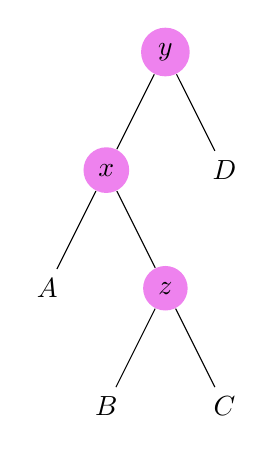
\begin{tikzpicture}
        \node[circle, fill=Violet] {$y$}
        child { 
            node[circle, fill=Violet] {$x$}
            child { node {$A$} }
            child {
                node[circle, fill=Violet] {$z$} 
                child { node {$B$} }
                child { node {$C$} }
            }
        }
        child { node {$D$} };
    \end{tikzpicture}
    $\longrightarrow$
    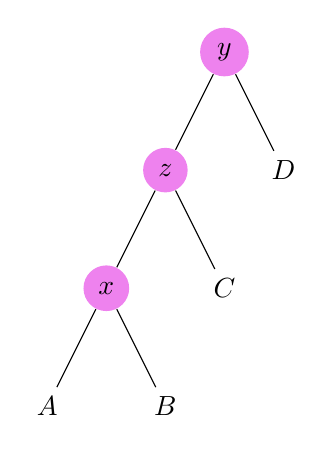
\begin{tikzpicture}
        \node[circle, fill=Violet] {$y$}
        child { 
            node[circle, fill=Violet] {$z$}
            child {
                node[circle, fill=Violet] {$x$}
                child { node {$A$} }
                child { node {$B$} }
            }
            child { node {$C$} }
        }
        child { node {$D$} };
    \end{tikzpicture}
    $\longrightarrow$
    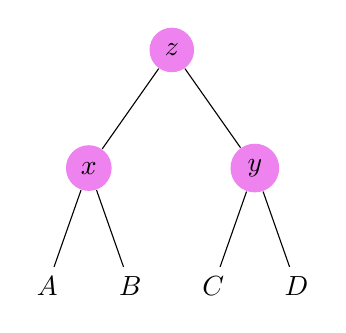
\begin{tikzpicture}[level 1/.style={sibling distance=6em}, level 2/.style={sibling distance=3em}]
        \node[circle, fill=Violet] {$z$}
        child {
            node[circle, fill=Violet] {$x$}
            child { node {$A$} }
            child { node {$B$} }
        }
        child {
            node[circle, fill=Violet] {$y$}
            child { node {$C$} }
            child { node {$D$} }
        };
    \end{tikzpicture}
    \caption{Double Left-Right Rotation}
\end{figure}

\begin{figure}[H]
    \tikzset{
        baseline = (current bounding box.center),
        level distance=3.5em
    }
    \centering
    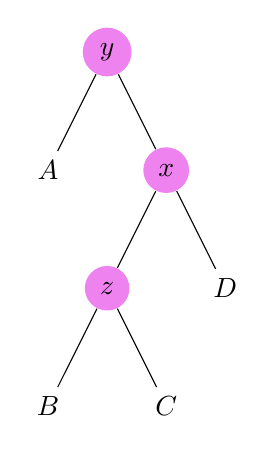
\begin{tikzpicture}
        \node[circle, fill=Violet] {$y$}
        child { node {$A$} }
        child { 
            node[circle, fill=Violet] {$x$}
            child {
                node[circle, fill=Violet] {$z$} 
                child { node {$B$} }
                child { node {$C$} }
            }
            child { node {$D$} }
        };
    \end{tikzpicture}
    $\longrightarrow$
    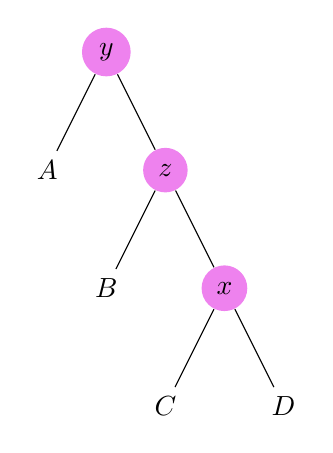
\begin{tikzpicture}
        \node[circle, fill=Violet] {$y$}
        child { node {$A$} }
        child { 
            node[circle, fill=Violet] {$z$}
            child { node {$B$} }
            child {
                node[circle, fill=Violet] {$x$}
                child { node {$C$} }
                child { node {$D$} }
            }
        };
    \end{tikzpicture}
    $\longrightarrow$
    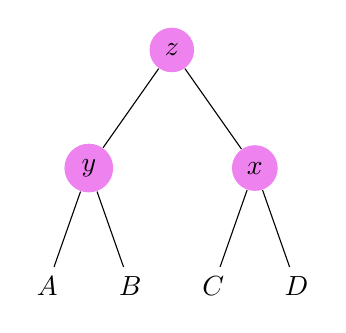
\begin{tikzpicture}[level 1/.style={sibling distance=6em}, level 2/.style={sibling distance=3em}]
        \node[circle, fill=Violet] {$z$}
        child {
            node[circle, fill=Violet] {$y$}
            child { node {$A$} }
            child { node {$B$} }
        }
        child {
            node[circle, fill=Violet] {$x$}
            child { node {$C$} }
            child { node {$D$} }
        };
    \end{tikzpicture}
    \caption{Double Right-Left Rotation}
\end{figure}

\subsection{\textsc{Insert}}

\begin{algorithm}[H] \begin{algorithmic}[1]
    \Procedure{AVL-Insert}{\textit{root}, $x$}
        \State \cmt{Insert $x$ into the tree at \textit{root}, return new root}
        \If {$\textit{root} = \text{NIL}$}
            \State $\textit{root} \gets \textsc{AVL\_Node}(x)$ \cmt{add $x$}
        \ElsIf {$x.\textit{key} < \textit{root.item.key}$}
            \State $\textit{root.left} \gets \textsc{AVL-Insert}(\textit{root.left}, x)$
            \State $\textit{root} \gets \textsc{AVL-Balance-Right}(\textit{root})$
        \ElsIf {$x.\textit{key} > \textit{root.item.key}$}
            \State $\textit{root.right} \gets \textsc{AVL-Insert}(\textit{root.right}, x)$
            \State $\textit{root} \gets \textsc{AVL-Balance-Left}(\textit{root})$
        \Else \cmt{$x.\textit{key} = \textit{root.item.key}$}
            \State $\textit{root.item} \gets x$ \cmt{replace with $x$}
        \EndIf
        \State \Return $\textit{root}$
    \EndProcedure
\end{algorithmic} \end{algorithm}

\subsection{\textsc{Delete}}

\begin{algorithm}[H] \begin{algorithmic}
    \Procedure{AVL-Delete}{\textit{root}, $x$}
        \State \cmt{Delete $x$ from the tree at \textit{root}, return new root}
        \If {$\textit{root} = \text{NIL}$}
            \State pass \cmt{$x$ not in tree}
        \ElsIf {$x.\textit{key} < \textit{root.item.key}$}
            \State $\textit{root.left} \gets \textsc{AVL-Delete}(\textit{root.left}, x)$
            \State $\textit{root} \gets \textsc{AVL-Balance-Left}(\textit{root})$
        \ElsIf {$x.\textit{key} > \textit{root.item.key}$}
            \State $\textit{root.right} \gets \textsc{AVL-Delete}(\textit{root.right}, x)$
            \State $\textit{root} \gets \textsc{AVL-Balance-Right}(\textit{root})$
        \Else {~} \cmt{$x.\textit{key} = \textit{root.item.key}$}
            \If {$\textit{root.left} = \text{NIL}$}
                \State $\textit{root} \gets \textit{root.right}$ \cmt{could be NIL}
            \ElsIf {$\textit{root.right} = \text{NIL}$}
                \State $\textit{root} \gets \textit{root.left}$
            \Else 
                \If {$\textit{root.left.height} > \textit{root.right.height}$}
                    \State $\textit{root.item}, \textit{root.left} \gets \textsc{AVL-Delete-Max}(\textit{root.left})$
                \Else
                    \State $\textit{root.item}, \textit{root.right} \gets \textsc{AVL-Delete-Min}(\textit{root.right})$
                \EndIf
            \EndIf
            \State $\textit{root.height} \gets 1 + \textsc{Max}(\textit{root.left.height}, \textit{root.right.height})$
        \EndIf
        \State \Return $\textit{root}$
    \EndProcedure
\end{algorithmic} \end{algorithm}

\begin{algorithm}[H] \begin{algorithmic}
    \Procedure{AVL-Del-Max}{\textit{root}}
        \State \cmt{Delete the maximum item from the tree at \textit{root}, return new root and deleted item}
        \Require $\textit{root} \neq \text{NIL}$
        \If {$\textit{root.right} = \text{NIL}$}
            \State \Return $\textit{root.item}, \textit{root.left}$
        \Else
            \State $\textit{item}, \textit{root.right} \gets \textsc{AVL-Delete-Max}(\textit{root.right})$
            \State $\textit{root} \gets \textsc{AVL-Balance-Right}(\textit{root})$
            \State \Return $\textit{item}, \textit{root}$
        \EndIf
    \EndProcedure
\end{algorithmic} \end{algorithm}

\subsection{Rebalancing}

\begin{algorithm}[H] \begin{algorithmic}[1]
    \Procedure{AVL-Balance-Left}{\textit{root}}
        \Require $\textit{root} \neq \text{NIL}$
        \State \cmt{First, recalculate height}
        \State $\textit{root.height} \gets 1 + \textsc{Max}(\textit{root.left.height}, \textit{root.right.height})$
        \State \cmt{Then, rebalance the left, if necessary}
        \If {$\textit{root.right.height} > \textit{root.left.height} + 1$}
            \State \cmt{Check for double rotation}
            \If {$\textit{root.right.left.height} > \textit{root.right.right.height}$}
                \State $\textit{root.right} \gets \textsc{AVL-Rotate-Right}(\textit{root.right})$
            \EndIf
            \State $\textit{root} \gets \textsc{AVL-Rotate-left}(\textit{root})$
        \EndIf
        \State \Return $\textit{root}$
    \EndProcedure
\end{algorithmic} \end{algorithm}

\begin{algorithm}[H] \begin{algorithmic}[1]
    \Procedure{AVL-Rotate-Left}{\textit{parent}}
        \Require $\textit{parent} \neq \text{NIL}$, $\textit{parent.right} \neq \text{NIL}$
        \State \cmt{Rearrange references}
        \State $\textit{child} \gets \textit{parent.right}$
        \State $\textit{parent.right} \gets \textit{child.left}$
        \State $\textit{child.left} \gets \textit{parent}$

        \State \cmt{Update heights; parent first because it is now deeper}
        \State $\textit{parent.height} \gets 1 + \textsc{Max}(\textit{parent.left.height}, \textit{parent.right.height})$
        \State $\textit{child.height} \gets 1 + \textsc{Max}(\textit{child.left.height}, \textit{child.right.height})$

        \State \cmt{Return new parent}
        \State \Return $\textit{child}$
    \EndProcedure
\end{algorithmic} \end{algorithm}

\section{Hashing}

\listu {
    \item Universe $U$\index{Hash Table!Universe}

    The set of all keys. We assume that $|U|$ is very large.
    
    \item Hash Table $T$\index{Hash Table}

    An array of fixed size $m$. Each location $T[i]$ is called a \term{bucket}\index{Hash Table!bucket}.

    \item Hash Function $h$\index{Hash Table!hash function}
    
    The hash function $h: U \rightarrow \{0, 1, \ldots, m-1\}$ maps each key in $U$ to an index in $\{ 0, 1, \dots, m - 1 \}$. For each key $k \in U$, $h(k)$ is called the \term{home bucket}\index{Hash Table!home bucket} of $k$.

    To access item with key $k$, examine $T[h(k)]$.
}

A hash table is an effective data structure for implementing dictionaries. Although \textsc{Search} for an element in a hes table can take as long as searching for an element in a linked list -- $\Theta(n)$ time in the worst case -- in practice, hashing preforms extremely well. Under reasonable assumptions, the average time to search for an element in a hash table is $\mathcal{O}(1)$. 

\subsection{Direct Access Table}

Direct addressing is a simple technique that works well when the universe $U$ of keys is reasonably small. If $U$ is small, then we can use an array $T$ of size $|U|$ to implement a dictionary, called a \term{direct access table}\index{Hash Table!Direct Access Table}. The key $k$ is used as an index into $T$ to access the item with key $k$.

\subsection{Hash Table}

The downside of direct addressing is apparent: if the universe $U$ is large or infinite. storing a table $T$ of size $|U|$ is impractical, and the set $K$ of keys \itblue{actually stored} may be so small relative to $Y$ that most of the space allocated for $T$ would be wasted. Instead, we use a hash table. 

{~~~}

However, when $m << |U|$, collisions are unavoidable. A \term{collision}\index{Hash Table!collision} occurs when two keys $k_1$ and $k_2$ (with $k_1 \neq k_2$) are mapped to the same bucket $h(k_1) = h(k_2)$. There are two ways to handle collisions: \term{open addressing}\index{Hash Table!Open Addressing} and \term{closed addressing / chaining}\index{Hash Table!Closed Addressing / Chaining}.

\subsubsection{Open Addressing}

In open addressing, if $T[h(k)]$ is occupied, then we search for the next available location in $T$ to store the item with key $k$. We call the original hash function $h_1$ the \term{primary hash function}\index{Hash Table!primary hash function}, such that $h_1(k)$ is the home bucket of $k$. We use the \term{probe sequence}\index{Hash Table!Probe Seuqnece} $h(k, i)$ to determine the bucket to try after $i$ collisions. 

\listu {
    \item \term{Linear Probing}\index{Hash Table!open addressing!linear probing}

    $h(k, i) = (h_1(k) + i) \mod m$

    Note that long clusters of occupied buckets can occur.

    \item \term{Quadratic Probing}\index{Hash Table!open addressing!quadratic probing}

    $h(k, i) = (h_1(k) + c_1i + c_2i^2) \mod m$

    $c_1$ and $c_2$ are constants dependent on $m$. 

    \item \term{Double Hashing}\index{Hash Table!open addressing!double hashing}

    $h(k, i) = (h_i(k) + i \cdot (h_2(k))) \mod m$, where $h_2(k)$ is a secondary hash function. 
}

\subsection{Close Addressing / Chaining}

In close addressing, we use a linked list to store the items in each bucket. Each nonempty slot points to a linked list, and all the elements that hash to the same slot go into that slot's linked list. 

The average-case performance of the hash table depends on how evenly the hash function $h$ distributes the keys across the buckets in the table. The \term{simple uniform hashing assumption}(SUHA)\index{Hash Table!Simple Uniform Hashing Assumption} states that any given key is equally likely to hash into any of the $m$ slots of the table, independently of where any other elements has hashed to. Under this assumption, the expected number of keys in each bucket is the same. 

The expected number of keys in a bucket is $\frac{n}{n}$, where $n$ is the number of items in the table and $m$ is the size of the table. This ratio is called the \term{load factor}\index{Hash Table!load factor} of the hash table, and we denote it by $\alpha$.
\chapter{Dynamic Array}

C styled arrays are static, meaning that they have a fixed size. In this chapter, we will learn how to implement a dynamic array, which is a data structure that can grow and shrink in size.

\begin{verbatim}
class DynamicArray {
    capacity: integer  # room for elements
    size:     integer  # actual number of elements
};
\end{verbatim}

\begin{minipage}[t]{0.4\linewidth} \begin{algorithm}[H] \begin{algorithmic}[1]
    \label{algo:da_insert}
    \Procedure{Insert}{$A, x$}
        \If{$A.size = A.capacity$}
            \State $A \gets \textsc{Resize}(A)$
        \EndIf
        \State $A.size \gets A.size + 1$
        \State $A[A.size] \gets x$
    \EndProcedure
\end{algorithmic} \end{algorithm} \end{minipage}
\hfill
\begin{minipage}[t]{0.5\linewidth} \begin{algorithm}[H] \begin{algorithmic}[1]
    \Procedure{Resize}{$A$}
        \State $B \gets \textsc{DynamicArray}(2 \times A.capacity)$
        \For {$i = 1$ \textbf{to} $A.size$}
            \State \textsc{Insert}($B, A[i]$)
        \EndFor
        \State \Return $B$
    \EndProcedure
\end{algorithmic} \end{algorithm} \end{minipage}

{~~~}

To analyze the running time of the above algorithm, see \hyperref[exam:amortized_accounting]{this example} using accounting method for amortized analysis. The amortized running time of the above algorithm is $\Theta(1)$.
\chapter{Graphs}

\begin{figure}[H]
    \tikzset{ every node/.style={draw, circle, minimum size=2em} }
    \centering
    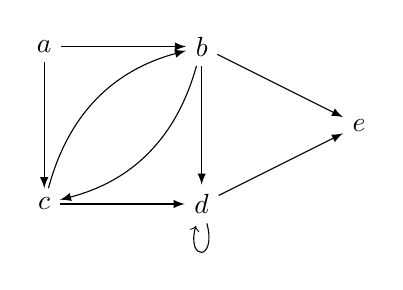
\begin{tikzpicture}[every edge/.style={draw, -latex}] 
        \node (a) at (0,0) {$a$};
        \node (b) at (2,0) {$b$};
        \node (c) at (0,-2) {$c$};
        \node (d) at (2,-2) {$d$};
        \node (e) at (4,-1) {$e$};

        \path (a) edge (b)
              (a) edge (c)
              (b) edge[bend left] (c)
              (b) edge (d)
              (b) edge (e)
              (c) edge[bend left] (b)
              (c) edge (d)
              (d) edge[loop below] (d)
              (d) edge (e);
    \end{tikzpicture}
    \hfil
    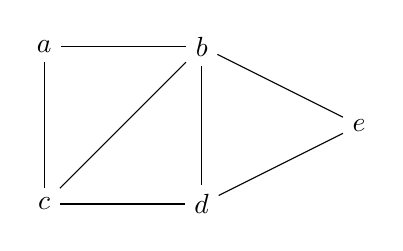
\begin{tikzpicture}
        \node (a) at (0,0) {$a$};
        \node (b) at (2,0) {$b$};
        \node (c) at (0,-2) {$c$};
        \node (d) at (2,-2) {$d$};
        \node (e) at (4,-1) {$e$};

        \path (a) edge (b)
              (a) edge (c)
              (b) edge (c)
              (b) edge (d)
              (b) edge (e)
              (c) edge (d)
              (d) edge (e);
    \end{tikzpicture}
\end{figure}

\section{Graphs}

\subsection{Graphs}

Define a graph $G = \{ V, E \}$

\subsubsection{Representations}

\listu {
    \item Adjacency matrix
    
    \begin{center} \begin{tabular}{c | c c c c c}
            & $a$ & $b$ & $c$ & $d$ & $e$ \\ \hline
        $a$ & 0   & 1   & 1   & 0   & 0   \\
        $b$ & 1   & 0   & 1   & 1   & 1   \\
        $c$ & 1   & 1   & 0   & 1   & 0   \\
        $d$ & 0   & 1   & 1   & 0   & 1   \\
        $e$ & 0   & 1   & 0   & 1   & 0
    \end{tabular} \end{center}

    Complexity: let $n = |V|$ and $m = |E|$
    \listu {
        \item Space: $O(n^2)$
        \item Edge query: $\Theta(1)$ time
    }

    \item Adjacency list
    
    % TODO: add figure

    Complexity: let $n = |V|$ and $m = |E|$
    \listu {
        \item Space: $\Theta(n + m)$
        \item Edge query: $\Theta(n)$ in worst-case time
    }
}

\subsection{Breadth-First Search}

In breadth first search, we start at a source $s \in V$, and explore every vertex reachable from $a$, using only edges. 

\begin{figure}[H]
    \centering
    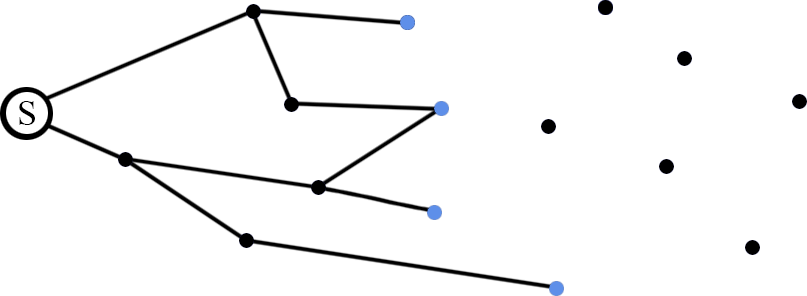
\includegraphics[width=0.5\linewidth]{images/BFS.png}
\end{figure}

We assign each vertex $v \in V$ a color, which can be one of the following:
\listu {
    \item White: $v$ has not been discovered
    \item Gray: $v$ has been discovered, but not explored
    \item Black: $v$ has been discovered and explored
}

Define $\pi[v]$ to be the predecessor of $v$ in the breadth-first search tree.

Define $d[v]$ to be the distance from $s$ to $v$ in the breadth-first search tree.

We use a queue to keep track of the vertices that we have discovered, but not yet explored.

\clearpage

\begin{algorithm}[H] \begin{algorithmic}[1]
    \Procedure{BFS}{$G$, $s$}
        \State \cmt{Initialize tracking info for all vertices}
        \For {$v \in G.V$}
            \State colour[$v$] = white
            \State $\pi[v] \gets \text{NIL}$
            \State $d[v] \gets \infty$
        \EndFor

        \State \cmt{Initialize empty queue and source vertex tracking info}
        \State $Q \gets \textsc{Make-queue}()$
        \State $\text{colour}[s] \gets \text{gray}$
        \State $\pi[s] \gets \text{NIL}$
        \State $d[s] \gets 0$
        \State \textsc{Enqueue}($Q$, $s$)

        \State \cmt{Main loop. Loop Invariant: $Q$ contains all (and only) gery vertices}
        \While {$Q \neq \textsc{Empty-queue}$}
            \State $u \gets \textsc{Dequeue}()$
            \For {$v \in G.Adj[u]$}
                \If {$\text{colour}[v] \gets \text{white}$}
                    \State $\text{colour}[v] \gets \text{gray}$
                    \State $\pi[v] \gets u$
                    \State $d[v] \gets d[u] + 1$
                    \State \textsc{Enqueue}($Q$, $v$)
                \EndIf
            \EndFor
            \State $\text{colour}[u] = \text{black}$
        \EndWhile
    \EndProcedure
\end{algorithmic} \end{algorithm}

In breath first search, \listu {
    \item Each vertex is enqueued at most once
    \item Each vertex is dequeued at most once
    \item Each adjacent list is examined at most once
    \item The time complexity is $\Theta(n + m)$
}

\subsubsection*{BFS Finds Shortest Paths}

Define $\delta(s, v)$ to be the length of the shortest path from vertex $s$ to vertex $v$ (i.e. the smallest number of edges in any path from $s$ to $v$). If there is no path from $s$ to $v$, then $\delta(s, v) = \infty$. Note that this definition will change when we consider \bred{weighted} graphs.

\theorem { 
    \label{thm:bfs-shortest-path} 
    Let $G = \{ V, E \}$ be a graph, and let $s \in V$. Then, after \textsc{BFS}($G$, $s$), $\forall v \in V$, $\delta(s, v) = d[v]$
}

To prove this theorem, we will need to prove the following lemmas first.

\lemma {
    \label{lem:bfs-shortest-path-1}
    $\forall (u, v) \in E$, $\delta(s, v) \leq \delta(s, u) + 1$
}

\begin{proof}
    (idea)

    If $\delta(s, u) = \infty$, then the claim holds trivially. 

    If $\delta(s, u) \neq \infty$, then $u$ is reachable from $s$.

    Thus, $v$ is also reachable from $s$.

    Thus, the shortest path from $s$ to $v$ is no longer than the shortest path from $s$ to $u$, plus the edge $(u, v)$.

    Hence, $\delta(s, v) \leq \delta(s, u) + 1$.
\end{proof}

\lemma {
    \label{lem:bfs-shortest-path-2}
    At ant point during BFS, $\forall v \in V$, $d[v] \geq \delta(s, v)$
}

\begin{proof}
    (idea)

    Use induction on the number of \textsc{Enqueue} operations.

    Immediately after we do the first \textsc{Enqueue} operation, $d[s] = 0$, and $\delta(s, s) = 0$.

    We also have $d[v] = \infty$, and $\delta(s, v) = \infty$ for all $v \in V - \{ s \}$.

    Now, consider some vertex $v$ that is first discovered while visiting a vertex $u$.

    By the IH, we have $d[u] \geq \delta(s, u)$.

    Hence, $d[v] = d[u] + 1 \geq \delta(s, u) + 1$ by Lemma 4.2.1. %TODO: use \ref

    Then $v$ is painted grey and $d[v]$ is not changed for the rest of the algorithm.
\end{proof}

\lemma {
    \label{lem:bfs-shortest-path-3}
    If $Q = \left< v_1, \dots, v_r \right>$, then $d[v_i] \leq d[v_{i+1}]$ for all $i \in \{ 1, \dots, r-1 \}$ and $d[v_r] \leq d[v_1] + 1$
}

\begin{proof}
    (sketch)

    Use induction on the number of \textsc{Dequeue} / \textsc{Enqueue} operations.

    When $Q = \left< s \right>$, the claim holds trivially.

    To prove the inductive step, we need to show that the lemma hold after applying \textsc{Dequeue} / \textsc{Enqueue} to $Q = \left< v_1, \dots, v_3 \right>$.

    \begin{itemize}
        \item Case 1
        
        If we perform a \textsc{Dequeue} operation, then $Q = \left< v_2, \dots, v_3 \right>$ afterwards.

        By the IH, $d[v_r] \leq d[v_1] + 1$ and $d[v_1] \le d[v_2]$.

        Hence, $d[v_r] \leq d[v_2] + 1$.

        All other inequalities are unaffected. 

        \item Case 2 
        
        If we perform a \textsc{Enqueue} operation, then $Q = \left< v_1, \dots, v_{r+1} \right>$ afterwards.

        We discover $v_{r+1}$ while visiting some vertex $u$, so $d[v_{r+1}] = d[u] + 1$.

        Vertex $u$ must have been the previous vertex dequeued from the queue. 

        Hence, either $v_1$ was discovered while visiting $u$, in which case $[v_1] = d[u] + 1$, or $Q$ was equal to $\left< u_2, v_1, \dots \right>$ at some prior point, in which case $d[u] \leq d[v_1]$ by IH.

        Hence, $d[v_{r+1}] = d[u] + 1 \leq d[v_1] + 1$.

        Otherwise, $d[v_r] \leq d[u] + 1 = d[v_{r+1}]$ by the IH. 
    \end{itemize}
\end{proof}

Now, we can prove the theorem.

\begin{proof}
    To derive a contradiction, suppose $d[v] \neq \delta(s, v)$ for some vertex $v \in V$.

    Suppose $v$ is a vertex with minimal $\delta(s, v)$ for which this is satisfied.

    By Lemma 4.1.2, we have $d[v] > \delta(s, v)$.

    % TODO: add a figure

    Because we chose $v$ with minimal $\delta(s, v)$, we have $d[u] = \delta(s, u)$.

    Hence, $d[v] > \delta(s, v) = \delta(s, u) + 1 = d[u] + 1$.

    Consider the colour of $v$ when we first dequeue $u$ from $Q$.

    \begin{itemize}
        \item If $v$ is painted \textbf{white}, then we set $d[v] = d[u] + 1$, which is a contradiction.
        \item If $v$ is painted \textbf{black}, then $v$ was in the queue before $u$. By Lemma 4.1.3, we have $d[v] \le d[u]$, which is a contradiction.
        \item If $v$ is painted \textbf{grey}, then $v$ was discovered while visiting some vertex $w$ that was dequeued earlier than $u$. Hence, $d [v] = d[w] + 1$, and by Lemma 4.1.3 we have $d[w] \le d[u]$. So $d[v] \le d[u] + 1$, which is a contradiction.
    \end{itemize}
\end{proof}

\subsubsection{Time complexity of BFS}

\listu {
    \item Initialization (painting vertices white, setting entries of $d$ to $\infty$ and entries of $\pi$ to NIL) takes $\Theta(|V|)$ time. 
    \item After initialization, we never paint a vertex white.
    \item Thus, each vertex is enqueued/dequeued at most once. 
    \item Hence, we spend $\mathcal{O}(|V|)$ time doing queue operations. 
    \item Every time we dequeue a vertex, we scan its out-neighbourhood to discover its neighbours:
    \listu {
        \item With an \textbf{adjacency list}, we consider each edge at most once (or at most twice in an undirected graph), so in total we need at most $\mathcal{O}(|E|)$ time to consider all of the edges.
        \item With an adjacency matrix, we scan each row of the matrix at most once, so in total we need at most $\mathcal{O}(|V|^2)$ time to consider all of the edges.
    }
}

\begin{minipage}[t]{0.45\linewidth} \begin{center}
    Using adjacency list: $\mathcal{O}(|V| + |E|)$
\end{center} \end{minipage}
\begin{minipage}[t]{0.45\linewidth} \begin{center}
    Using adjacency matrix: $\mathcal{O}(|V|^2)$
\end{center} \end{minipage}

\subsection{Depth-First Search}

\listu {
    \item In DFS, we walk through the graph as far as possible until we hit a dead end -- when this happens, we backtrack to an undiscovered vertex. 
    \item Similar to BFS, we paint vertices as we go: 
    \listu {
        \item Painted white: undiscovered
        \item Painted grey: discovered but not yet visited 
        \item Painted black: visited
    }
    \item Instead of storing distances/depths, we store timestamps: 
    \item \listu {
        \item $\textit{disc}[v] = \null$time at which $v$ is first discovered
        \item $\textit{vis}[v] = \null$time at which we finish visiting $v$
    }
}

\listu {
    \item One approach is to simply replace the \itblue{queue} from the BFS algorithm with a \itblue{stack}. This gives us an \bred{iterative} DFS algorithm. 
    \item However, it is more natural to write DFS as a recursive algorithm.
}

\begin{minipage}[t]{0.45\linewidth} \begin{algorithm}[H] \begin{algorithmic}[1]
    \Procedure{DFS}{G}
        \State \cmt{Initialization}
        \For {each $v \in G.V$}
            \State $d[v] \gets f[v] \gets \infty$
            \State $\pi[v] \gets \text{NIL}$
        \EndFor
        \State $\text{time} \gets 0$  \cmt{global}
        \State \cmt{Main loop}
        \For {each $v \in G.V$}
            \If {$d[v] = \infty$} 
                \State \cmt{colour[$v$] = white}
                \State \Call{DFS-Visit}{$G$, $v$}
            \EndIf
        \EndFor
    \EndProcedure
\end{algorithmic} \end{algorithm} \end{minipage}
\hfill
\begin{minipage}[t]{0.45\linewidth} \begin{algorithm}[H] \begin{algorithmic}[1]
    \Procedure{DFS-Visit}{$G$, $v$}
        \State \cmt{Discovered (colour[v] = grey)}
        \State $d[v] \gets \text{time} \gets \text{time} + 1$
        \State \cmt{Do something with $v$, if desired}
        \State \cmt{Explore $v$'s adjacency list}
        \For {each $u \in G.adj[v]$}
            \If {$d[u] = \infty$} 
                \State \cmt{colour[$u$] = white}
                \State $\pi[u] = v$
                \State \Call{DFS-Visit}{$G$, $u$}
            \EndIf
        \EndFor
        \State \cmt{Finished (colour[$v$] = black)}
        \State $f[v] \gets \text{time} \gets \text{time} + 1$
    \EndProcedure
\end{algorithmic} \end{algorithm} \end{minipage}

\subsubsection{DFS Forests}

We classify each edge $(u, v)$ based on the colour of $v$ when we consider this edge:

\listu {
    \item \term{Tree edges} are the edges $u$, $v \in E$ that form the DFS forest stored by $\pi$ 
    
    The vertex $v$ is painted \bred{white} when $(u, v)$ is considered 

    \item \term{Back edges}\index{DFS Tree!Back Edge} are the edges $(u, v) \in E$ such that $v$ is an ancestor of $u$ in the DFS forest 
    
    The vertex $v$ is painted \bred{grey} when $(u, v)$ is considered

    \item \term{Forward edges}\index{DFS Tree!Forward Edge} are the edges $(u, v) \in E$ such that $v$ is a descendant of $u$ in the DFS forest 
    
    The vertex $v$ is painted \bred{black} when $(u, v)$ is considered

    \item \term{Cross edges}\index{DFS Tree!Cross Edge} are all other edges $(u, v) \in E$ that are not part of the DFS forest (i.e. $v$ is neither an ancestor nor a descendant of $u$)

    The vertex $v$ is painted \bred{black} when $(u, v)$ is considered
}

\begin{figure}[H]
    \centering
    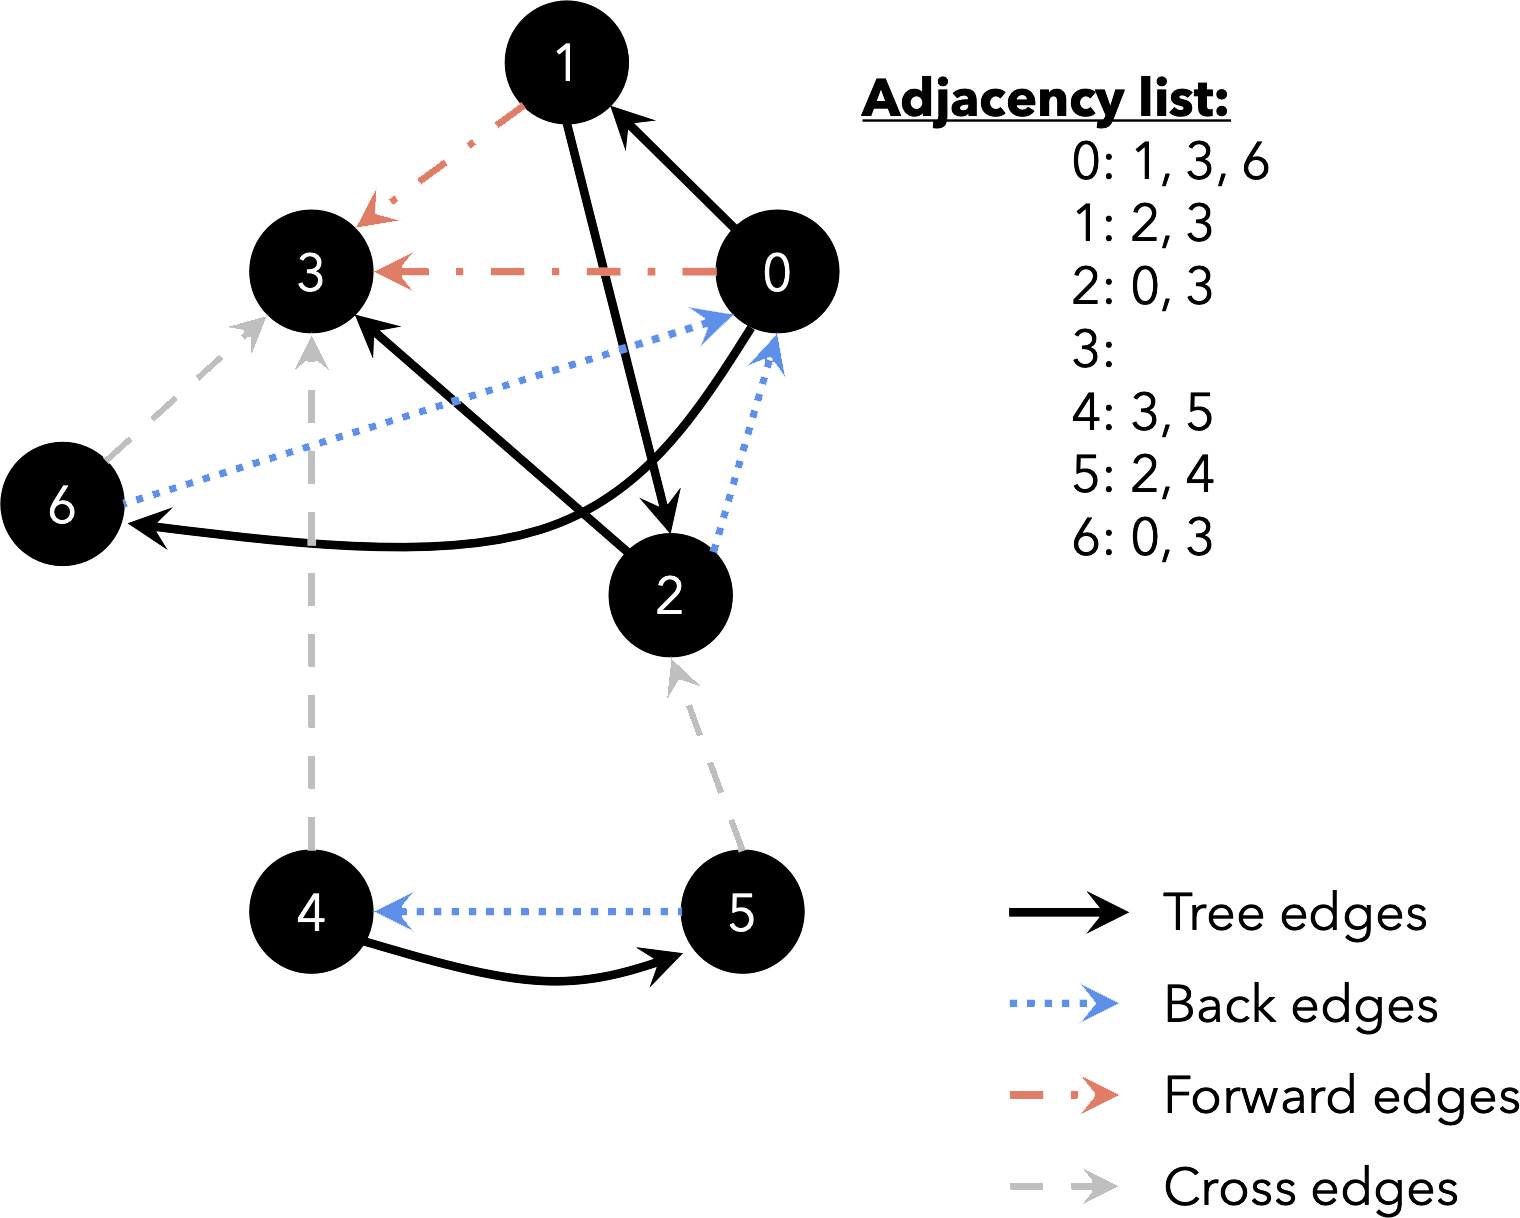
\includegraphics[width=0.5\linewidth]{images/DFS-Tree_Edges.png}
\end{figure}

Note that for undirected graphs, there are NO forward edges and NO cross edges.

\subsubsection{Time Complexity}

The run-time of DFS is similar to BFS.

\begin{minipage}[t]{0.45\linewidth} \begin{center}
    Using adjacency list: $\mathcal{O}(|V| + |E|)$
\end{center} \end{minipage}
\begin{minipage}[t]{0.45\linewidth} \begin{center}
    Using adjacency matrix: $\mathcal{O}(|V|^2)$
\end{center} \end{minipage}

\subsubsection{Parenthesis theorem}\index{Parenthesis Theorem}

\theorem {
    After performing \textsc{DFS}$(G = (V, E))$, for any two vertices $u$, $v \in V$, exactly one of the following statements holds:
    \listo {
        \item The intervals $\left[ \textit{disc}[u], \textit{vis}[u] \right]$ and $\left[ \textit{disc}[v], \textit{vis}[v] \right]$ are disjoint, and neither $u$ nor $v$ is a descendant of the other in the DFS forest.
        \item The interval $\left[ \textit{disc}[u] , \textit{vis}[u] \right]$ is contained entirely in the interval $\left[ \textit{disc}[v], \textit{vis}[v] \right]$, and $u$ is a descendant of $v$ in the DFS forest.
        \item The interval $\left[ \textit{disc}[v], \textit{vis}[v] \right]$ is contained entirely in the interval $\left[ \textit{disc}[u], \textit{vis}[u] \right]$, and $v$ is a descendant of $u$ in the DFS forest.
    }
}

\begin{proof}
    (sketch)

    Suppose that $\textit{disc}[u] < \textit{disc}[v]$.

    \listu {
        \item Case 1: $\textit{disc}[v] < \textit{vis}[u]$

        \begin{center} 
            \includegraphics*[width=0.2\linewidth]{images/Parenthesis-Thm-Grey-u.png}

            $v$ is first discovered while $u$ is painted grey.  
        \end{center}

        So $v$ is a descendant of $u$.

        We don't backtrack to $u$ until we have finished visiting $v$.

        Therefore, we paint $v$ black and set $\textit{vis}[v]$ before backtracking to $u$. Hence, $\textit{vis}[v] < \textit{vis}[u]$.

        \item Case 2: $\textit{vis}[u] < \textit{disc}[v]$

        \begin{center} \includegraphics*[width=0.2\linewidth]{images/Parenthesis-Thm-Black-u.png}

            $v$ is first discovered while $u$ is painted black.  
        \end{center}

        So $v$ is not a descendant of $u$.

       Since $\textit{disc}[u] < \textit{dics}[v]$, $u$ is not a descendant of $v$.

       Since $\textit{disc}[u] < \textit{vis}[u]$ and $\textit{disc}[v] < \textit{vis}[v]$, we have $\textit{disc}[u] < \textit{vis}[u] < \textit{disc}[v] < \textit{vis}[v]$.
    }

    When $\textit{disc}[v] < \textit{disc}[u]$, proof is symmetric.
\end{proof}

\subsection{Strongly connected}

Recall that an undirected graph is connected if and only if there is a path of edges between any pair of vertices in $V$. What about directed graphs? A directed graph $G = (V, E)$ is strongly connected if and only if, for all $u$, $v \in V$, there is a path of edges from $u$ to $v$ in $G$. 

\begin{figure}[H]
    \centering
    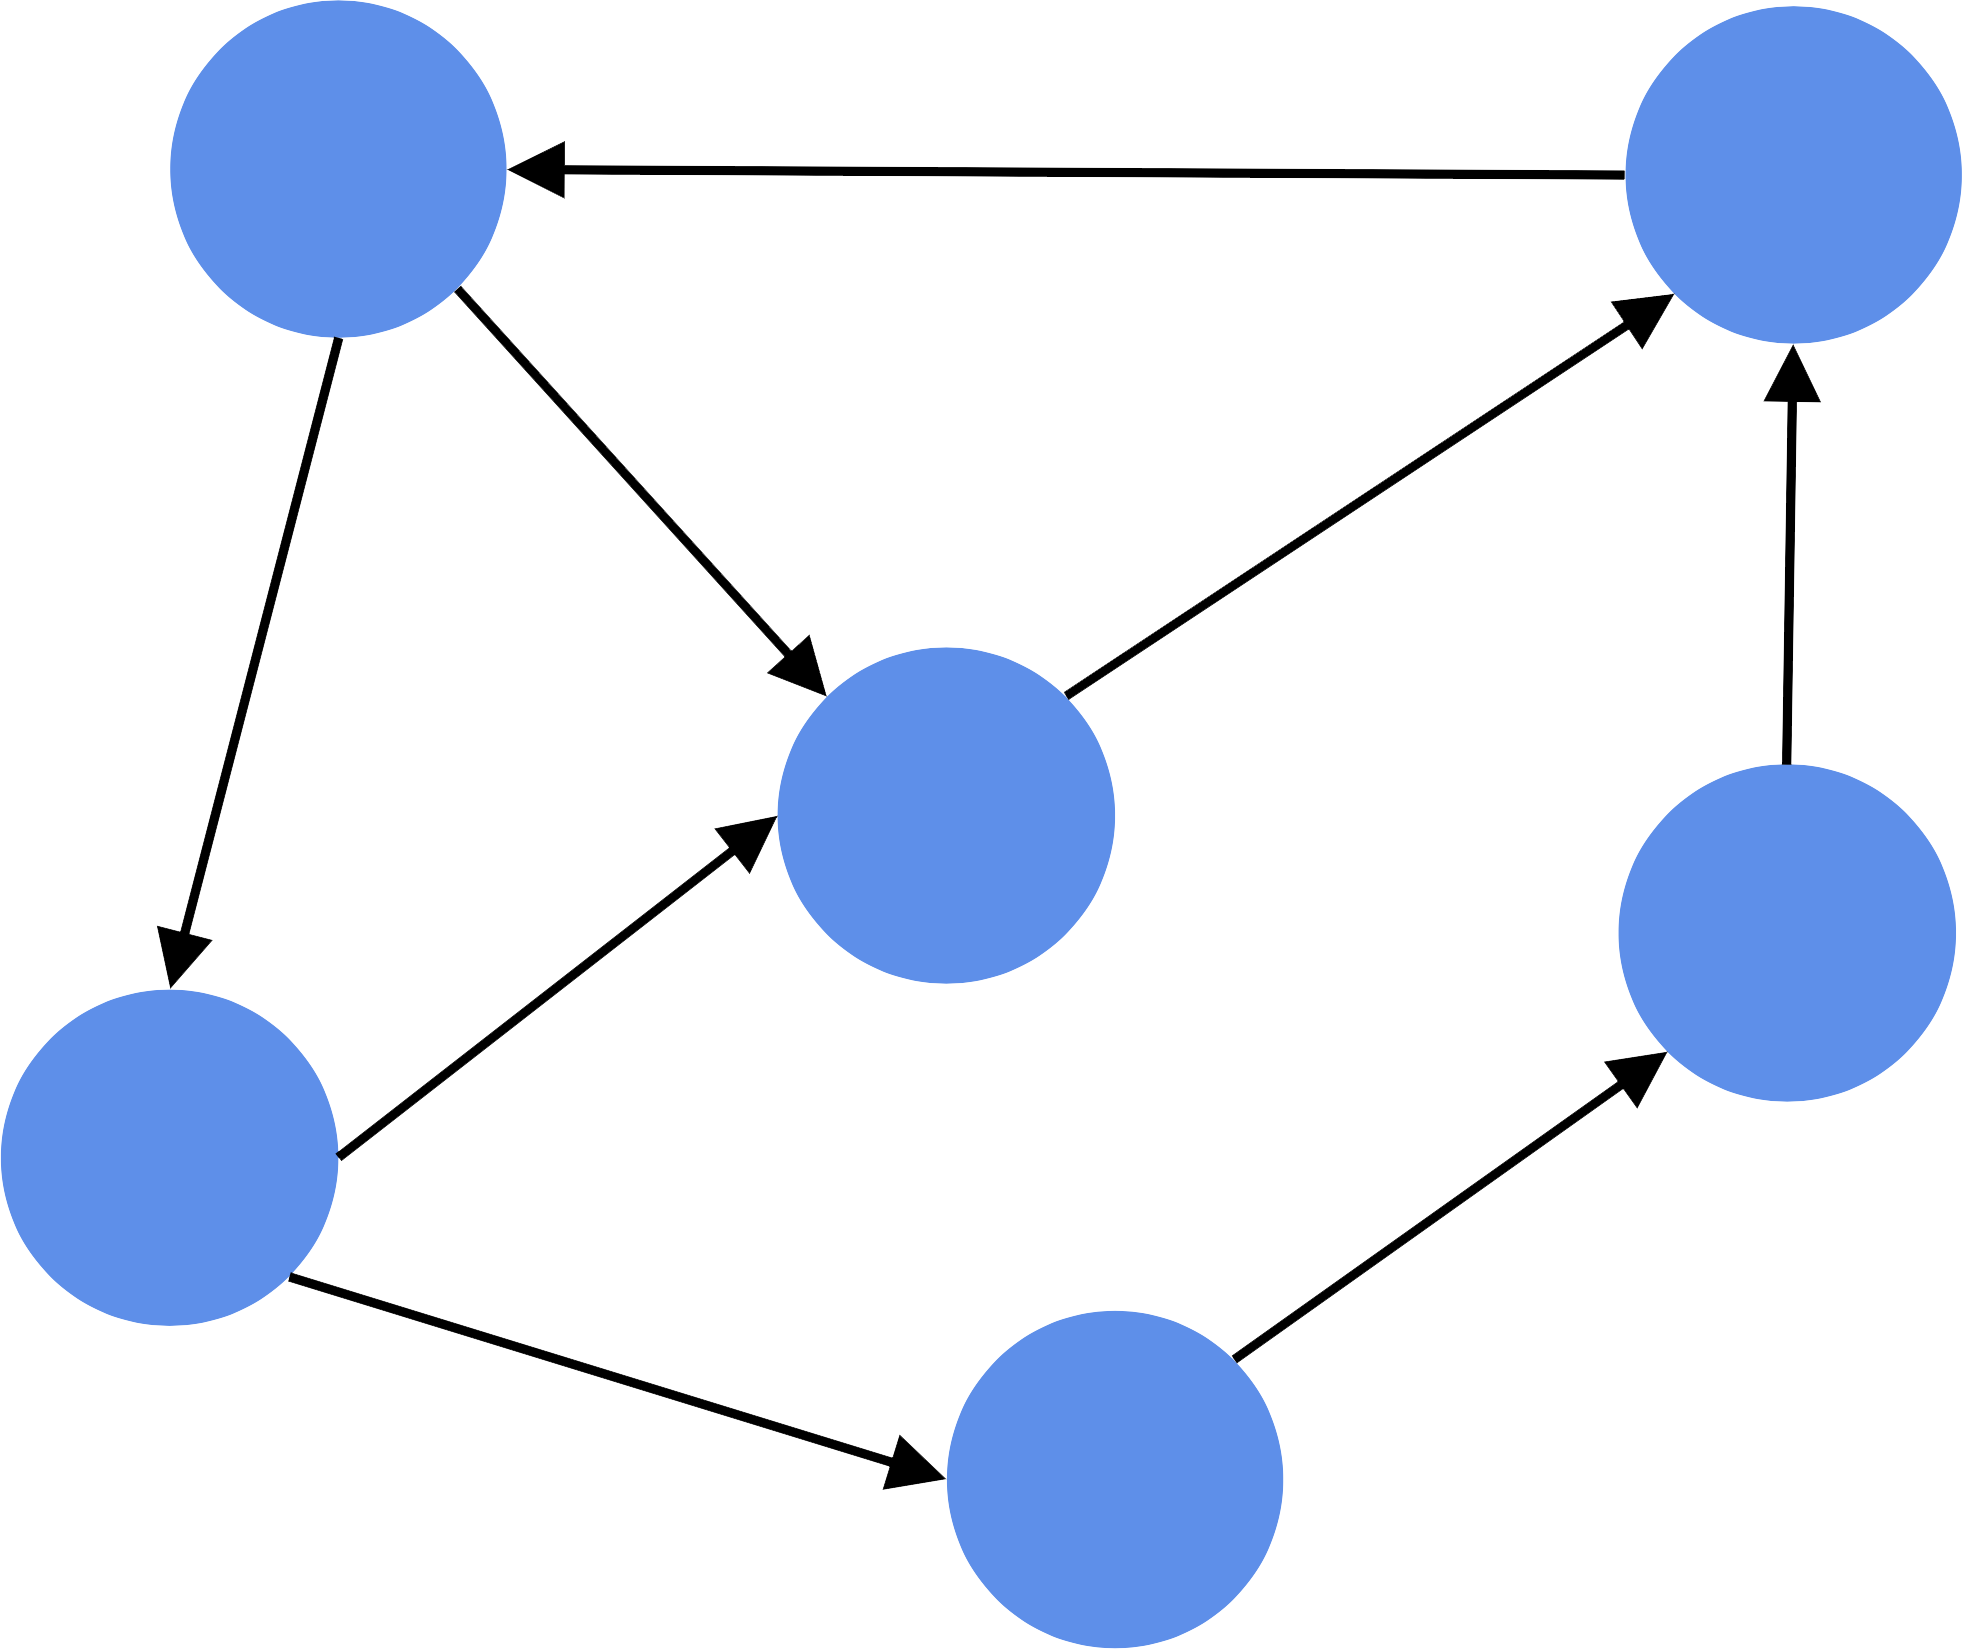
\includegraphics[width=0.2\linewidth]{images/Strongly-Connected.png}
    \qquad
    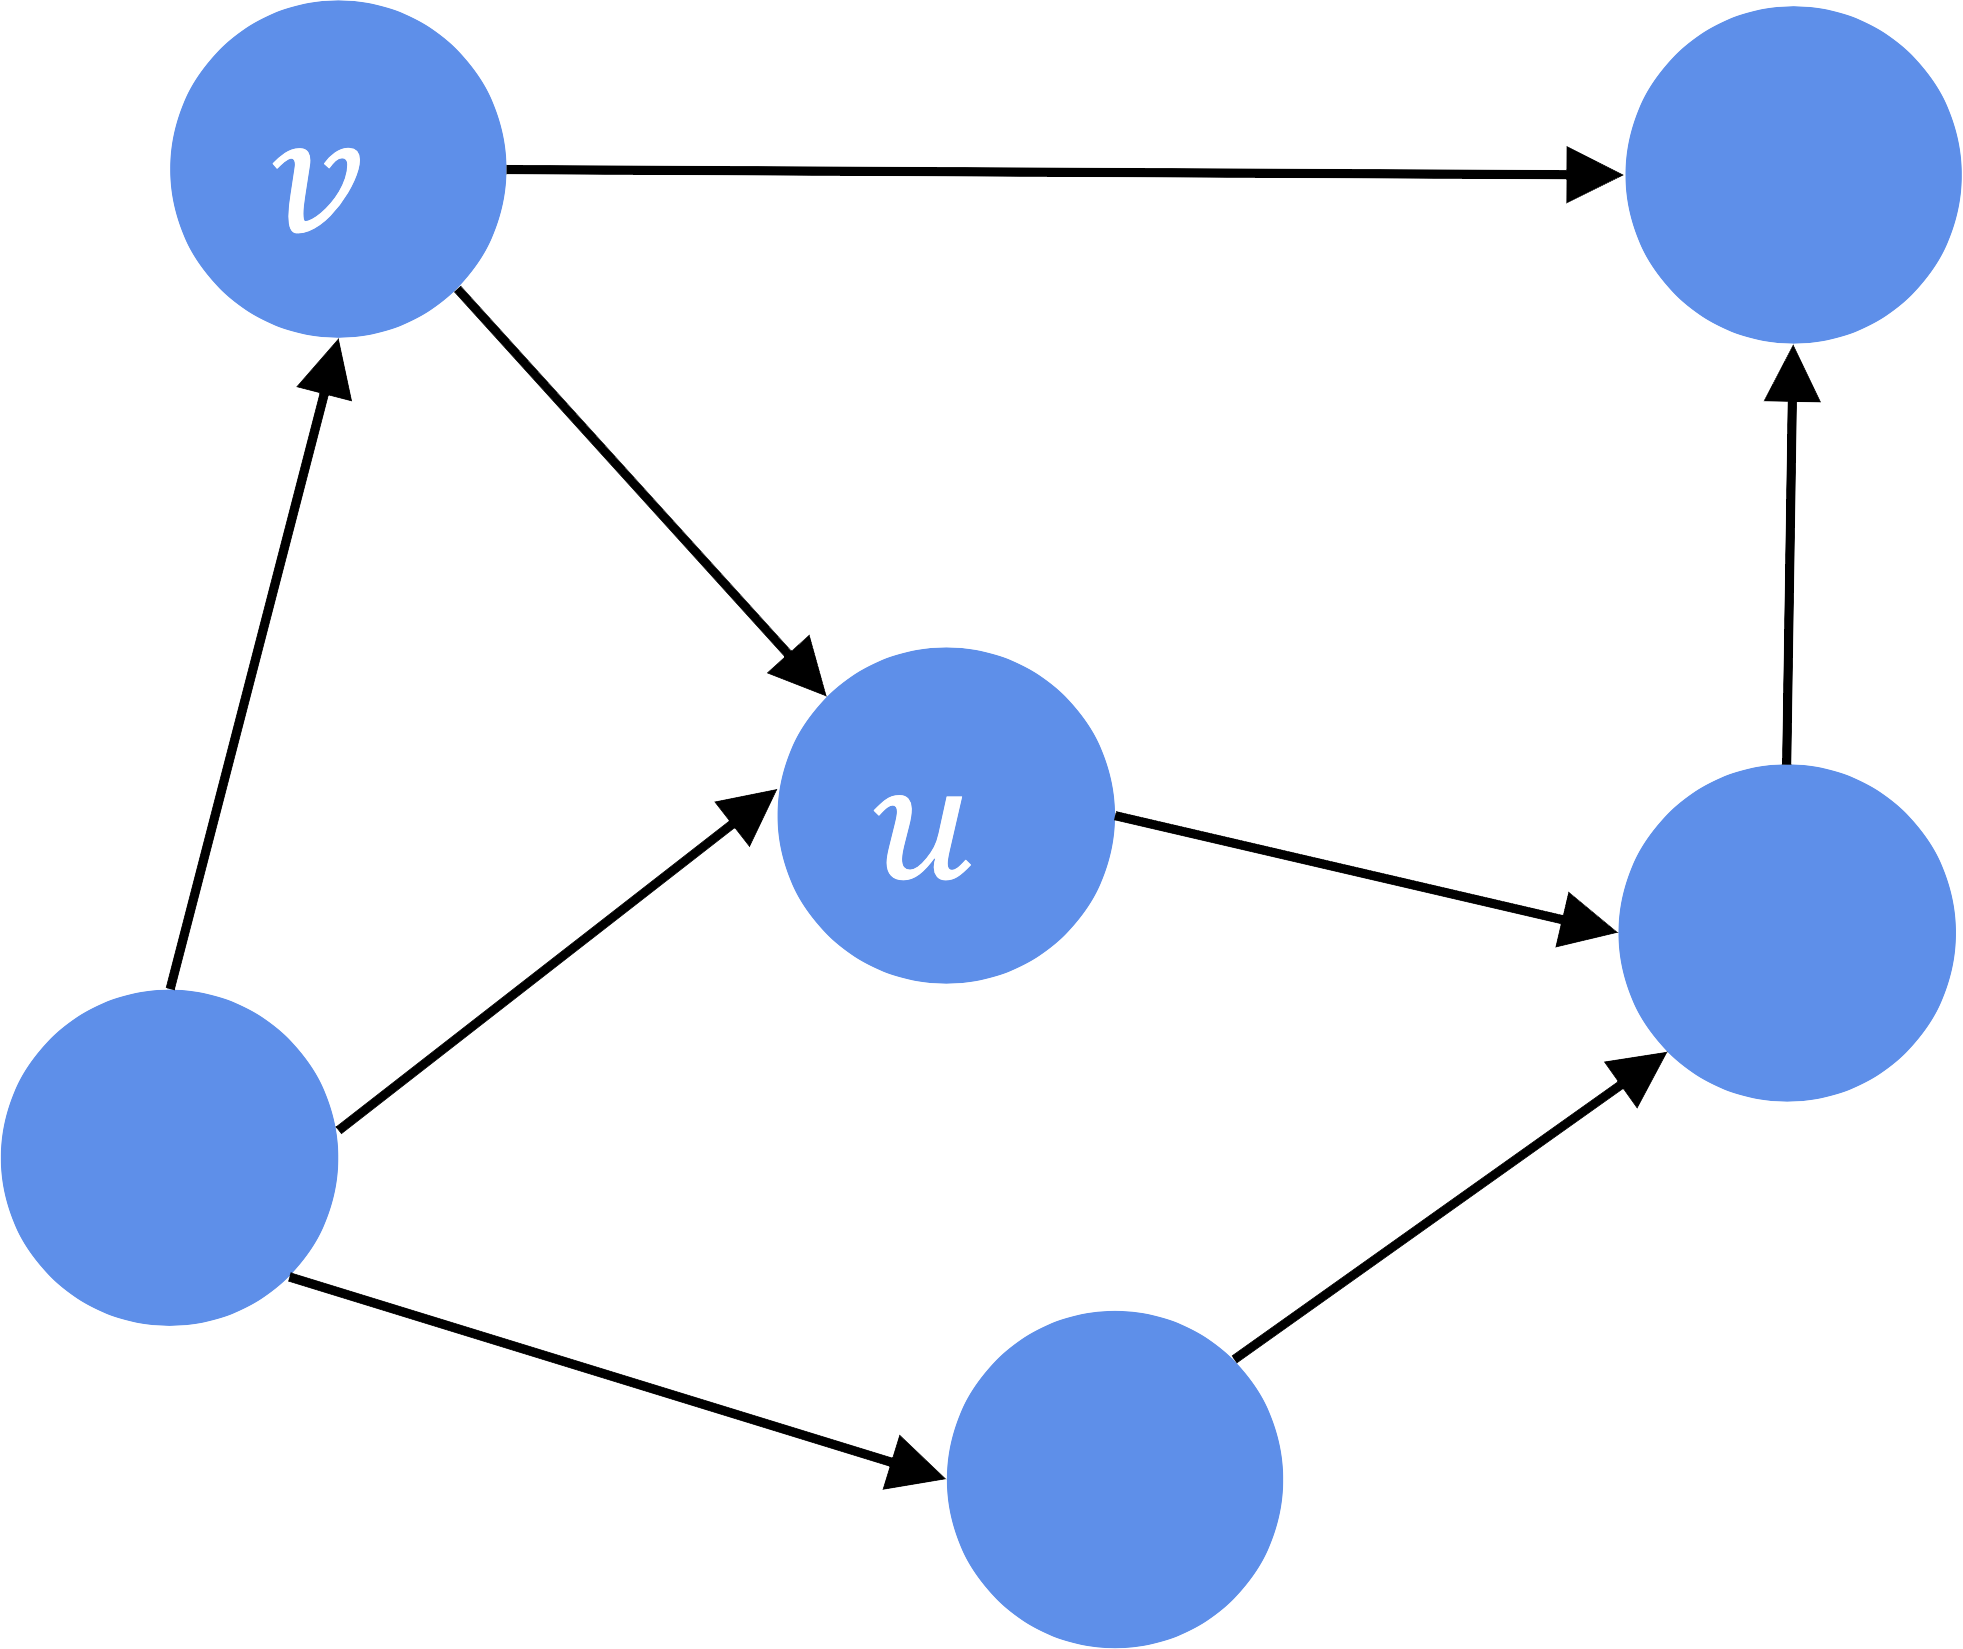
\includegraphics[width=0.2\linewidth]{images/Not-Strongly-Connected.png}
    \caption*{A strongly connected graph (left) and a non-strongly connected graph (right, where $v$ is not reachable from $u$)}
\end{figure}

\listu {
    \item Run \textsc{DFS} on the \bred{transpose} of $G$ (reverse edge direction of all edges in $G$)
    \item \itblue{Reorder} vertices in decreasing order of finish time (in $G.V$ and within each adjacency list)

    Run \textit{DFS} on $G$ using the new ordering of vertices

    \item Each DFS tree is one strongly connected component
}

\section{Minimum Spanning Trees}

\section{Disjoint Sets}

\part{Algorithms}
\chapter{Sorting}

\section{Heap Sort}

\section{Quick Sort}

\begin{algorithm}[H] \begin{algorithmic}[1]
    \Procedure{QuickSort}{$A$}
        \If $\textsc{Len}(A) \le 1$ 
            \State \Return $A$
        \EndIf
        \State $L, p, G \gets \textsc{Partition}(A)$
        \State \Return $\textsc{QuickSort}(L) + [p] + \textsc{QuickSort}(G)$
    \EndProcedure
\end{algorithmic} \end{algorithm}

\subsection{Deterministic Quick Sort}

In deterministic quick sort, we choose the pivot to be a certain index in the array. We can choose the pivot to be the first element, the last element, or the middle element. 

\listu {
    \item Run-time depends on input ordering
    \item Bad ordering would yield bad run-time, while random ordering would generally yield better run-time
}

\subsection{Randomized Quick Sort}

In randomized quick sort, we choose the pivot to be a random index in the array. Intuitively, the expected run-time would be the same as deterministic quick sort -- $\Theta(n \lg n)$ -- but the worst case run-time would be much better.

\part{Analysis}
\chapter{Average Case Analysis}

In \term{average case analysis}\index{Average Case Analysis}, we are interested in the average performance of an algorithm. we take the average, or the expected value, over the distribution of the possible inputs. 

For each $n$, define $S_n = \{ \text{all inputs of size } n \}$, and if we consider the inputs to be random, then $S_n$ is the sample space. For each $x \in S_n$, define $P(x)$ to be the probability that $x$ will be chosen as the input. Define $t(x)$ as the number of steps preformed on input $x$. $t$ is the random variable. 

Then, the average case running time is defined as $$\begin{aligned}[t]
    T(n) & = E[t]                           \\
         & =\sum_{x \in S_n} P(x) \cdot t(x)
\end{aligned}$$

\example {
    Consider the linear search algorithm on a linked list $L$. 

    \begin{algorithm}[H] \begin{algorithmic}[1]
        \Procedure{LinSearch}{$L$, $x$}
            \State $z \gets L.\textit{head}$
            \While{$z \neq \text{NIL}$ \textbf{and} $z.\textit{data} != x$}
                \State $z \gets z.\textit{next}$
            \EndWhile
            \State \Return $z$
        \EndProcedure
    \end{algorithmic} \end{algorithm}

    Let $S_n$ be the sample space of all linked lists of size $n$. Let $P(x)$ be the probability that $x$ is chosen as the input. Let $t(x)$ be the number of steps performed on input $x$.

    \listu {
        \item We need to know $S_n$ with probability

        Consider the inputs $\texttt{input}_1 = ([1, 2, 3], 2)$ and $\texttt{input}_2 = ([``a", ``b", ``c"], ``b")$, note that they will take the same steps. We only need one input for each possible value of $t$.

        Define $S_n = \{ ([1, 2, \dots, n], 1), ([1, 2, \dots, n], 2), \dots, ([1, 2, \dots, n], n), ([1, 2, \dots, n], 0) \}$. 

        \item We assume all the inputs happen equally likely, then $P(x) = \frac{1}{n+1}$.
        
        \item  We need an exact formula for $t(x)$.
        
        In practice, we choose some ``key operations'' s.t. counting \bred{only} these operations is within a constant factor of total time -- then set $t(x) = \text{number of key operations}$. 

        Here, we choose line 3, $z.\textit{data} \neq x$, as the key operation.
    }

    Then, we have $\begin{aligned}[t]
        T(n) & = \sum_{(L, i) \in S_n} t(L, i) \cdot P(L, i)                            \\
             & = \frac{1}{n + 1} \sum_{i = 0}^n t([1, 2, \dots, n], i)                  \\
             & = \frac{1}{n + 1} \left( t([1, 2, \dots, n], 0) + \sum_{i=1}^n i \right) \\
             & = \frac{1}{n + 1} \left(n + \frac{n(n + 1)}{2} \right)                   \\
             & = \frac{n}{n + 1} + \frac{n}{2} 
    \end{aligned}$
}

\example { \allowdisplaybreaks
    Consider $\textsc{Search}(T, k)$ on a hash table $T$ for a key $k$. 

    Assume $t$ has $m$ slots, and uses chaining to resolve collisions. Assume that prior to applying the textsc{Search} algorithm, the hash table contains $n$ keys. 

    Assume the key $k$ is samples uniformly at random from $U$. 

    Let $N(k)$ be the number of keys examined during search for $k$. $N(k)$ is the key operation. 

    \begin{align*}
        E[N(k)]                    & = \sum_{k \in U} P[k] \cdot N(k)                     \\
                                   & = \sum_{i=0}^{m-1} \sum_{\substack{k \in U           \\
        h(k) = i}} P[k] \cdot N(k) & \text{regroup terms}                                 \\
                                   & \le \sum_{i=0}^{m-1} \sum_{\substack{k \in U         \\
        h(k) = i}} P[k] \cdot L_i  & \text{since } N(k) \le L_i \text{ when } h(k) = i    \\
                                   & = \sum_{i=0}^{m-1} L_i \cdot \sum_{\substack{k \in U \\
        h(k) = i}} P[k]                                                                   \\
                                   & = \sum_{i=0}^{m-1} L_i \cdot P[h(k) = i]             \\
                                   & = \sum_{i=0}^{m-1} L_i \cdot \frac{1}{m}             \\
                                   & = \frac{1}{m} \sum_{i=0}^{m-1} L_i                   \\
                                   & = \frac{n}{m}
    \end{align*}
}

\example {
    Consider \textsc{QuickSort} on an array $A$ of size $n$.

    Let $S_n = \{ \text{all permutations of } [1, 2, dots, n] \}$

    We assume an uniform distribution of the inputs, then $P(x) = \frac{1}{n!}$.

    Let the random variable $T(A)$ be the total number of comparisons between elements of $A$.

    Define $X_{i, j} = \begin{cases}
        1 & \text{if } i \text{ is compared to } j \\
        0 & \text{otherwise}
    \end{cases}$ for $1 \le i < j \le n$.

    Then, $\displaystyle T(A) = \sum_{i=1}^{n-1} \sum_{j=i+1}^n X_{i, j}$.

    The probability $\begin{aligned}[t]
        P(X_{i,j} = 1) & = P(i \text{ or } j \text{ appear in } A \text{ before all other values in range } [i...j]) \\
                       & =\frac{1}{j - i + 1} + \frac{1}{j - i + 1}                                                  \\
                       & = \frac{2}{j - i + 1}
    \end{aligned}$

    Then, $\begin{aligned}[t]
        E[T(A)] & = \sum_{i=1}^{n-1} \sum_{j=i+1}^n E[X_{i,j}]           \\
                & = \sum_{i=1}^{n-1} \sum_{j=i+1}^n P(X_{i,j} = 1)       \\
                & = \sum_{i=1}^{n-1} \sum_{j=i+1}^n \frac{2}{j - i + 1}  \\
                & = \sum_{i=1}^{n-1} \sum_{j=i+1}^n \frac{2}{\alpha + 1}
                & \text{substitute } j - i \text{ with } \alpha          \\
                & < \sum_{i=1}^{n-1} \sum_{j=i+1}^n \frac{2}{k}          \\
                & = \sum_{i=1}^{n-1} \Theta(\lg n)                       \\
                & = \Theta(n \lg n)
    \end{aligned}$
}
\chapter{Amortized Analysis}\index{Amortized Analysis}

In amortized analysis, we analyze the cost of a sequence of operations, not just a single operation. The amortized cost of a sequence of operations is the average cost per operation. 

\begin{figure}[H]
    \centering
    \begin{tikzpicture}
        \fill[MyBlue] (0em,0em) rectangle ++(0.9em,0.9em);
        \fill[MyRed]  (1em,0em) rectangle ++(0.9em,2em  );
        \fill[MyBlue] (2em,0em) rectangle ++(0.9em,0.9em);
        \fill[MyBlue] (3em,0em) rectangle ++(0.9em,0.9em);
        \fill[MyRed]  (4em,0em) rectangle ++(0.9em,4em  );
        \fill[MyBlue] (5em,0em) rectangle ++(0.9em,0.9em);
        \fill[MyBlue] (6em,0em) rectangle ++(0.9em,0.9em);
        \fill[MyBlue] (7em,0em) rectangle ++(0.9em,0.9em);
        \fill[MyBlue] (8em,0em) rectangle ++(0.9em,0.9em);
        \fill[MyRed]  (9em,0em) rectangle ++(0.9em,8em );
        \fill (10.25em,0.5em) circle (0.125em);
        \fill (10.625em,  0.5em) circle (0.125em);
        \fill (11em,0.5em) circle (0.125em);
        %
        \node at (1em,6.5em) {infrequent, \textbf{\color{MyRed}expensive} operations};
        \node at (4.5em,-3em) {frequent, \textbf{\color{MyBlue}cheap} operations};
        \draw[MyRed,-latex] (0.5em,5.5em)  -- (1.5em,2.5em);
        \draw[MyRed,-latex] (1.25em,5.5em) -- (4.5em,4.5em);
        \draw[MyRed,-latex] (2em,7.5em)    -- (8.5em,8em);
        \draw[MyBlue,-latex] (2em,-2.25em) -- (0.5em,-0.5em);
        \draw[MyBlue,-latex] (2.75em,-2.25em) -- (2.5em,-0.5em);
        \draw[MyBlue,-latex] (3.5em,-2.25em) -- (3.5em,-0.5em);
        \draw[MyBlue,-latex] (4.25em,-2.25em) -- (5.5em,-0.5em);
        \draw[MyBlue,-latex] (4.5em,-2.25em) -- (6.5em,-0.5em);
        \draw[MyBlue,-latex] (5em,-2.25em) -- (7.5em,-0.5em);
        \draw[MyBlue,-latex] (5.75em,-2.25em) -- (8.5em,-0.5em);

        \fill[Violet] (12em,3em) rectangle ++(4.1em,1em);
        \fill[Violet] (16em,4.5em) -- (17em,3.5em) -- (16em,2.5em) -- cycle;

        \fill [MyOrange] (19em,0em) rectangle ++(0.9em,2.1em);
        \fill [MyOrange] (20em,0em) rectangle ++(0.9em,2.1em);
        \fill [MyOrange] (21em,0em) rectangle ++(0.9em,2.1em);
        \fill [MyOrange] (22em,0em) rectangle ++(0.9em,2.1em);
        \fill [MyOrange] (23em,0em) rectangle ++(0.9em,2.1em);
        \fill [MyOrange] (24em,0em) rectangle ++(0.9em,2.1em);
        \fill [MyOrange] (25em,0em) rectangle ++(0.9em,2.1em);
        \fill [MyOrange] (26em,0em) rectangle ++(0.9em,2.1em);
        \fill [MyOrange] (27em,0em) rectangle ++(0.9em,2.1em);
        \fill [MyOrange] (28em,0em) rectangle ++(0.9em,2.1em);
        %
        \draw[pen colour={MyOrange},, decorate, decoration = {calligraphic brace, amplitude = 1em}] (19em,2.7em) -- (29em,2.7em);
        \node[text width=11em] at (24em,6em) {``spread'' the expensive computations over the entire sequence};
    \end{tikzpicture}
\end{figure}

\listu {
    \item The \term{worst-case sequence complexicy}\index{Amortized Analysis!Worst-Case Sequence Complexity} of a sequence $S$ of $k$ operations is the maximum possible total steps performed by $S$ (taken over all possible inputs to the operations in $S$).

    \item The worst-case sequence complexity is \bred{at most} $k \times \null$the worst-case complexity of any individual operation in $S$.

    \item Suppose that the worst-case sequence complexity of a sequence of $k$ operations is $T(k)$. Then the (worst-case) \term{amortized complexity}\index{Amortized Analysis!Amortized Complexity} per operation of this sequence is $\frac{T(k)}{k}$.

    \item With amortized analysis, we take the average of the costs of multiple opertions (as opposed to average-case analysis, where we calculate the cost of a single operation by averaging over the input distribution)
}

\section{Aggregated Method}

In the \term{aggregated method}\index{Amortized Analysis!Aggregated Method}, we determine the upper bound $T(n)$ on the total cost of a sequence of $N$ operations, then calculate the average cost per operation as $\frac{T(n)}{n}$. 

\example {
    Consider when we insert into an array. We increase the size of the array by 4 when it is $\frac{3}{4}$ full. 

    For simplicity, suppose that each insert with no resizing requires $c$ steps, for some constant $c \in \mathbb{N}^+$ (so each insert with resizing requires $c \cdot n  + c$ steps, where $n$ is the number of items in the array prior to resizing).

    \begin{center} \begin{tabular}{c c}
        \centering
            Operation Number & Cost     \\
            \hline
            1                & $c$      \\
            2                & $c$      \\
            3                & $c$      \\
            4                & $4c$     \\
            5                & $c$      \\
            6                & $c$      \\
            7                & $c$      \\
            8                & $7c$     \\
            9                & $c$      \\
            10               & $10c$    \\
            $\vdots$         & $\vdots$
    \end{tabular} \end{center}

    Within a sequence of $k$ insertions, we need to resize $\floor{\frac{k - 1}{3}}$ times. For all $k$ insert operations, the total cost is $$T(k) = c \cdot \sum_{i=1}^{\floor{\frac{k-1}{3}}} (3i + 1) + c \cdot \left( k - \floor{\frac{k-1}{3}} \right)$$

    Note that $\begin{aligned}[t]
        c \cdot \sum_{i=1}^{\floor{\frac{k-1}{3}}} (3i + 1)
         & = c \cdot \sum_{i=1}^{\floor{\frac{k-1}{3}}} 3i + \sum_{i=1}^{\floor{\frac{k-1}{3}}} 1                                    \\
         & = 3c \cdot \sum_{i=1}^{\floor{\frac{k-1}{3}}} i + c \cdot \floor{\frac{k-1}{3}}                                           \\
         & = \frac{3}{2}c \cdot \floor{\frac{k-1}{3}} \cdot \left( \floor{\frac{k-1}{3}} + 1 \right) + c \cdot \floor{\frac{k-1}{3}}
           \in \Theta(k^2)
    \end{aligned}$
     
    Thus, $T(k)$ is $\Theta(k^2)$. The amortized cost per operation is $\frac{T(k)}{k} = \Theta(k)$.
}

\example {
    Consider a $k$ digit binary counter. 

    In this problem, we count the total number of bits changed in the counter. We can do this by counting the number of times each bit changes.

    \begin{center} \begin{tabular}{c c}
        Bit Number & Number of Changes       \\
        \hline
        0          & $m$                     \\
        1          & $\approx \frac{m}{2}$   \\
        2          & $\approx \frac{m}{4}$   \\
        $\vdots$   & $\vdots$                \\
        $i$        & $\approx \frac{m}{2^i}$ \\
        $\vdots$   & $\vdots$
    \end{tabular} \end{center}

    Then, $\begin{aligned}[t]
        T & = \sum_{i=0}^{(\lg m)-1} \frac{m}{2^i}       \\
          & = m \cdot \sum_{i=0}^{(\lg m)} \frac{1}{2^i} \\
          & < m \sum_{i=0}^{\infty} \frac{1}{2^i}        \\
          & = 2m
    \end{aligned}$
}

\section{Accounting Method}

The \term{accounting method}\index{Amortized Analysis!Accounting Method} is a form of aggregate analysis which assigns to each operation an amortized cost which may differ from its actual cost. Early operations have an amortized cost higher than their actual cost, which accumulates a saved ``credit'' that pays for later operations having an amortized cost lower than their actual cost. Because the credit begins at zero, the actual cost of a sequence of operations equals the amortized cost minus the accumulated credit. Because the credit is required to be non-negative, the amortized cost is an upper bound on the actual cost. Usually, many short-running operations accumulate such credit in small increments, while rare long-running operations decrease it drastically.

\example {
    \label{exam:amortized_accounting}
    Consider a sequence of $m$ \hyperref[algo:da_insert]{\textsc{Insert}} for dynamic array.

    Recall that the ``cost'' is the actual run-time, while the ``charge'' is the estimated amortized time.

    Note that for $k = 2^n + 1$, we need $2^n = k - 1$ for reading and $2^n + 1 = k$ for writing. Thus, the cost is $2k + 1$.

    Then, we know that $\text{cost}(\textsc{Insert}(k)) = \begin{cases}
        2k + 1 & \text{if } k = 2^n + 1 \\
        1      & \text{otherwise}
    \end{cases}$

    Define $\text{charge}(\textsc{Insert}(k)) = \$5$. We need $\$1$ for writing the new element, and save $\$4$ as credit. 

    We need to prove our credit invariant: every element in the second half of the array has $\$4$ credit.

    \begin{proof}
        Proof by induction on the number of operations done. 

        \begin{itemize}
            \item init: $0$ elements, $0$ credits
            \item Consider one \textsc{Insert}
            Assuming credit invariant holds

            \begin{itemize}
                \item If the array does not grow, then the new element gets $\$4$ credit. The credit invariant holds.
                \item If the array does grow, it must be full, the total credits is $\$4 \cdot \frac{n}{2} = \$2n$, enough toi cover copying $n$ elements. The new element gets $\$4$ credit. The credit invariant holds.
            \end{itemize}
        \end{itemize}
    \end{proof}

    Thus, $\begin{aligned}[t]
        \text{Amortized} \le \frac{\text{WCSC}}{m} & = \frac{\text{total cost}}{m}      \\
                                                   & \le \frac{\text{total charge}}{m}
                                                   & \text{because of credit invariant} \\
                                                   & = \frac{5m}{m}                     \\
                                                   & = 5
    \end{aligned}$
}

\part{Appendices}

\chapter*{Bibliography}
% \addcontentsline{toc}{chapter}{\textcolor{ocre}{Bibliography}}

\section*{Books}
% \addcontentsline{toc}{section}{Books}
\printbibliography[heading=bibempty,type=book]

%----------------------------------------------------------------------------------------
%	INDEX
%----------------------------------------------------------------------------------------

\cleardoublepage
\phantomsection
\setlength{\columnsep}{0.75cm}
% \addcontentsline{toc}{chapter}{\textcolor{ocre}{Index}}
\printindex

\end{document}